\NewChapter{3}{3}

\counterwithin{figure}{section}

\begin{refsection}
\begin{center}
\hspace{}
\\[1.0 in]
Holistic Water Cycle Analysis via the Confluence of Climate Model, Satellite, \\
Ground Truth, and Machine Learning Signal Processing Technologies: Two \\
North American Transboundary River Watersheds

\\[1.0 in]

Albert Eric Larson \\ 
Soni Pradhanang \\
Thomas Boving \\ 
Ali Shafqat Akanda \\[1.0 in]
\emph{Prepared for submission to MDPI Water}



\end{center}
\newpage

\subsection{Abstract}
Water continuously cycles throughout the land, ocean, and atmosphere. Accordingly, it is important for hydrological analyses to consider water as it moves throughout the entire hydrosphere, and not just a single facet of the process. We use neural networks as a device to transform geospatial observations of water quantity and quality into forecasts of ground truth streamflow measurements. Two very large transboundary basins, the Columbia River and Yukon River, are subjects of this investigation. We first describe the basins. Then we create two datasets for each basin: one with coupled surface flow, subsurface flow, and sea surface temperature of the basin adjacent oceans; and another with simply the surface and subsurface flow land measurements constrained to the definitive boundaries of the delineated watershed. Finally, we load these datasets into Flux to Flow (F2F), our neural network test platform. Our results indicate that, even with the smallest neural network we try (four neurons only), use of sea surface temperature greatly improves forecasting of monthly streamflow from up to two years lag between the input images and the output gauged streamflow measurements. We see the future use of the F2F pattern having more output targets and likely requiring multiple compute nodes to scale the work. We discuss and identify drought monitoring as a suitable next step. We believe this work has only scratched the surface regarding the integration of land and ocean parameter datasets to fields devoid of non-numerical observations.

\subsection{Keywords}
water, water quantity, streamflow, sea surface temperature, GLDAS, MODIS, Columbia River, Yukon River, z-score, Nash Sutcliffe efficiency, neural networks

\subsection{Introduction}
Depending on the location, there are different water related signals that humans can witness and measure. These time variant water signals include but are not limited to parameters such as rainfall, snowfall, cloud cover, fog, ice, soil moisture, streamflow, river height, body of water temperature (lakes, seas, ponds, oceans), tidal timing and intensity, waterbody color, turbidity, and trace chemical concentrations in the water. These variables are commonly cloistered into variables of the land, variables of the atmosphere, and finally but certainly not least important variables of the ocean. Together they form the hydrosphere. We focus on variables of the land and variables of the ocean; however, we affirm the impact of the atmosphere upon land and ocean. Even at long time scales, there are certain parts of the globe that are constantly obscured from viewing with traditional bands of the electromagnetic spectrum due to noise such as clouds, wind, or other interference. This fact places an emphasis on the need for continuation of innovation in satellite measurements, ground sensors, and the spectrum of devices in between. The state of the science is still in many instances ‘flying blind’; Earth’s environment is dynamic and complex and modern solutions need to grow to combat modern problems. 

We consider two extra-large basins. As an added complexity, we target transboundary watersheds. The motivation behind the use of transboundary watersheds is to simulate differences or nuance when leaving the gates of our national data systems in the acquisition of gauged river discharge measurements. In this instance, our journey is a short one to the northern riparian of the United States: Canada. Our view considers seventeen years of data, spanning years at monthly snapshots as opposed to the shorter end of the time spectrum (seconds, minutes, hours, days, or weeks). The two basins selected herein (Yukon River, Columbia River) are unique because of, among other features, their: 1, far from equatorial latitude; 2, proximity to the integration of land and ocean; 3, great range in quantity of water infrastructure between the two habitats; 4, large range of elevation change.

We study surface and subsurface flow as computed for one of the GLDAS datasets. Additionally, we couple the two GLDAS datasets to MODIS sea surface temperature, creating a global dataset mostly devoid of non-number pixels. Of interest is the predictability of several gauges at a time when using the clipped version of GLDAS versus our custom ocean-enabled version of GLDAS. Furthermore, we modulate the lever of z-scored datasets versus non-z-scored datasets. We find that combining surface flow with subsurface flow (derived measurements of the changing weight of water in a region) and sea surface temperature has a markedly improved performance in predicting gauged streamflow than the datasets containing only surface and subsurface flow.

The wide lens guiding motivation behind this study is three-fold: 1, to improve the reader’s understanding and capability to ‘quickly’ visualize the pertinent available macroscopic modern water cycle monitoring data sets; 2, to highlight state of the science level data typically used by experts for the generation and interpretation of global policy targeted outputs; and 3, to present a narrative of water (hydrology, limnology, oceanography) as the focal point of study because of its status as a primary building block of life. 

\subsection{Materials \& Methods}
\subsubsection{Yukon River Watershed}
The Yukon River and greater watershed are situated within part of the state of Alaska, and the eponymously named Canadian territory known simply as Yukon (Figure \ref{fig3_1}). A thorough baseline hydrological artefact of the Yukon River exists (\cite{brabets2000environmental}). The headwaters of the Yukon River emerge from the constellation of finger style lakes (e.g., Atlin Lake, Marsh Lake, Teslin Lake, Gladys Lake) known customarily as the Southern Lakes region along the northwestern border of the Canadian province of British Columbia. Sampled along the route of the river, one is likely to find bedrock, confined and unconfined aquifers, a host of unique soil profiles, vegetation, permafrost, and a not to be understated flurry of flora and fauna friendly to subarctic climatology. At a microscopic, chemical level, the frequent boreal forest attributes concurrent with the frigid temperatures are well understood (\cite{o2010source}). Zooming out to a wider view than just the Yukon, evidence continuously mounts regarding the impacts of the changing climate. As goes the rest of the world, the Yukon feels an impulse. Nitrogen and phosphorous pollution are two of the more notorious organic chemical components that when unmanaged can wreak havoc on a watershed, causing eutrophication, loss of biodiversity (\cite{carpenter1998nonpoint}). It’s a short walk down the primrose path to a river lacking in a once endemic species of fish (\cite{kanter2020nitrogen}). 

The Yukon River is famous for its salmon. In the last several years, the Yukon has come under public scrutiny for declining populations of chinook and chum in the Yukon and its neighbor river the Kuskokwim. A combination of bycatch in pollack fisheries, overfishing, marine heatwaves and algae blooms are causing the environment to become potentially less suitable for fish. There are prevalent modern terrors such as “forever chemicals” and the ubiquity of microplastics in the hydrosphere to the degree that many careers are being dedicated to the study as it relates to contamination of our waterways (\cite{schreder2014flame}). It is a wonder at all sometimes that our river ways can sustain any life given the way some humans steward the gift. Humanity has much work to do to repair and improve the current status quo.

Environmental flows, or “e-flows” is “the quantity, timing, and quality of water flows required to sustain freshwater and estuarine ecosystems and the human livelihoods and wellbeing that depend on these ecosystems” (\cite{arthington2018brisbane}). Considering a perspective filtered through the comprehension of e-flows, the Yukon has natural advantages. It is in a higher latitude, close to the North Pole (there’s a town called North Pole in Alaska along the Yukon). Because of the high latitudes, constantly cold (equatorially relative) temperatures, and sometimes very long dark periods of time, there’s a tendency for life forms to shirk away from this environment. As such, the river is less prone to farming, heavy nutrient loading, or industry strain. That is not to say that its observation is in vain or without merit, far from it. Large swaths of previously unoccupied or lightly occupied land are important ones to observe with greater clarity the forcings and results of the natural global Earth phenomena as it is subjected to human intervention.

Physically, the Yukon River and surrounding land has all the features one desires in a naturally occurring surface water: beautiful lakes, high mountain scenery, sinuous meanders, novel woodland creatures. For example, erosion drives the creation of oxbow lakes, small slices of river cut off after anomalous water patterns drive unusual erosion in a suitable soil substrate. The Yukon is home to many cyclically migrating birds, as well as a habitat for many bears (\cite{sierraclubMeetIce}). Bears are attracted to the Yukon’s most notorious creatures: the chinook and chum populations traversing the watercourse. 

\subsubsection{Columbia River Watershed}
South of the Yukon Basin, at the southern edge of British Columbia and the boundary between the contiguous US and Canada lies the beginning of the Columbia River (Figure \ref{fig3_1}). The watershed is split into two major parts by the Cascade Mountain range running northerly from Oregon up into British Columbia. Land wise, the basin is primarily east of the Cascades. The western half of the larger Columbia drainage basin as divided by the Cascades finds a large share of water in the flows of the Willamette River. The waters of the Willamette stem from Waldo Lake, and it moves in a northerly direction before merging with the formal Columbia River. The Willamette unfortunately came under great scrutiny for the exhaustion of its goodwill to the point of receiving the designation of one of the United States most polluted waterways (\cite{lundin2019legacy}). There are efforts to restore the waterway that have logged twenty-five active years and are beginning to restore these damaged arteries and veins of water. 

The Willamette meets the Columbia in Portland, Oregon, and there is a short portion that flows north and west into the Pacific Ocean, catching a view of Mount Saint Helens to the east as the Columbia traces the boundary between the states of Oregon and Washington. Prior to Portland, the Columbia has a long meandering path through Washington and the Canadian province of British Columbia. Moving against the current, one follows the river in an easterly direction until coming upon the Tri-Cities in Washington. Kennewick, Pasco, and Richland are the three towns at the confluence of the Columbia and the other two of its other major tributaries (Snake River and Yakima River). All proverbial roads of the Columbia move upwards in elevation, and the coherence of a singular river eventually dissipates. Where Yakima for example weaves back into the Cascade Range, there are many finger lakes serving as the upper riparian. 

Snake River is the largest tributary of the Columbia, its starting line in Wyoming trekking a westward course just north of Bear River. The Snake River’s headwaters are outflows of Yellowstone. The Columbia River and Snake River share a potentially overlooked but crucial feature from their convergence backwards: a vector of hydraulic projects along both of their paths, none more notable than the Grand Coulee Dam (GCD). GCD is a hydroelectric power generating dam, with a power generating capacity of 6,809 megawatts (MW)). GCD is the largest power station (not just hydro, but of any type) in the United States. Though, it is dwarfed in size to the Chinese Three Gorges Dam, which boasts an installed capacity of 22,500 MW.

The eponymous Columbia ultimately has its headwaters in British Columbia where it forms from a series of three finger lakes: the smaller Slocan Lake and the protracted-in-length Upper Arrow Lake and Kootenay Lake. The three direct suppliers of water are amongst the Columbia Range of mountains. Furthering the point, there is also a Mount Columbia in the range.

\subsubsection{Data Sources}
This study compiles together several large portions of data from five different institutions. NASA provides the two land variables, surface and subsurface flow. These variables are derived by integrating several meteorological forcings into the Noah water balance algorithm. The Noah land surface model has a rich history dating back to the late 1980s with formal named implementations released in the middle 1990s (\cite{ek2003implementation}). Surface and subsurface flow are produced measurements of unit kilograms per square meter and represent the spatial weight of water at a given time in each location (\cite{xia2012comparative}). Noah factors known soil properties, solar radiation, precipitation, wind, pressure, humidity, and changes in the purses of snowpack (if applicable to the region). 

The sea surface temperature product used is one of the monthly outputs from the MODIS instrument on the Aqua satellite. In this instance, the thermal longer wave infrared band observed by MODIS is selected (\cite{nasaYears}). Furthermore, we use the data product that only looks at nighttime passes of the MODIS sensor. Daytime passes captured are ignored because of the potential diurnal warming effect that manifest in daytime observations. The skin of the ocean can become surficially inflated. Our preference is to a measurement of the ocean closer to the signature of the depths of the waters rather than the strength of the sun on a given day. Solar radiation is already encompassed in the calculation of land flows, so we attempt to limit its impact. 

Gauged streamflow for both basins are obtained through the United States Geological Survey and Canada’s bureau of climate and the environment (\cite{usgs2016national}; \cite{ecRealTimeHydrometric}). In all instances, we constrained ourselves to near continuous basin measurements over the entirety of the time series. The requirement of continuity (no non-number pixels and preferably no interpolation between months) plays a part in the quantity of measurements per basin. The study length is 210 single month measurements, beginning with July 2002 (coinciding with the first available monthly measurement of MODIS) and ending with December 2019. Measurements of actual streamflow in cubic feet per second for each basin are provided in the Figure \ref{fig3_2}.

\subsubsection{Preprocessing}
We run two distinct workflows across the time series for the Columbia and the Yukon basin. Motivated by a desire to understand whether the coupling of monthly SST to the GLDAS measurements of water flux across land impacts the speed and ability of the neural networks to learn algorithms connecting the inputs and outputs (i/o), we create datasets that are comprised just of surface and subsurface flow, and those that combine time aligned SST with the surface and subsurface flow measurements. 

The process of combining land and surface measurements is illustrated in Figure \ref{fig3_3}. In the top row, we have one measurement of surface (Qs) and subsurface (Qsb) flow. In the second row first column, we have added those two measurements together pixelwise. In the second column, second row, the combined Qs and Qsb are integrated with the corresponding monthly measurement of SST. In row two column two, having the single colormap representing all numbers provided causes a “washed out” effect where the Qs and Qsb measurements disappear because their physical range here are roughly between 0.0 and 1.0 kilograms per meter squared, as opposed to the wider 0.0 to 20.0°C range. Concurrently, row three captures the dynamic ranges of water flux over land, and the temperature of the ocean’s surface temperature.

In their respective raw formats, the land and ocean variables have different resolutions and different grids for each pixel of data. This fact makes assimilation of the data in its raw state impossible. The fix for this problem is bilinear regridding. We retain the MODIS grid and resolution of approximately 9 km x 9 km per pixel. To facilitate regridding, we utilize xESMF, a high level python package hooked into the Fortran, C, and C++ based Earth System Modeling Framework (\cite{zhuang2019xesmf}). We input the source image (Qs and Qsb), the destination grid (SST), and the type of regridding (bilinear). The algorithm provides as an output our source image in the destination grid.

We also use a windowing technique to eliminate nan values from the MODIS SST images. The PyTorch software suite has the function to create tiles of uniform smaller images from a large input (\cite{paszke2019pytorch}). We unfold each MODIS raster into smaller non-overlapping squares. Within each tile, we set the software to find any non-number values and replace them with the average of the available numerical values in the tile. One could simply take the mean of the entire global image and replace non-number values that way; however, this is prone to the creation of unusual bias due to the wide variance of sea surface temperature based on location of observation. By using this tile method, we limit potential bias through the consideration of pixels only that are in relative proximity to each other. After gap filling, we fold the tiles back up into the original image size.

Our control preprocessing in the study follows the same chain found in the first iteration of Flux to Flow. We clip the measurements of Qs and Qsb to the geographical constraints captured in the publicly available shapefiles for each basin. To do this, we involve a few different publicly available software packages. We open the shapefile (a digital vector storage format) with GeoPandas (\cite{jordahl2020geopandas}), convert the vector file to a GeoJSON file with shapely, and clip each measurement of surface and subsurface flow with rasterio (\cite{gillies2019rasterio}) and xarray (\cite{hoyer2017xarray}). As opposed to the coupled land and ocean images, we do not add the measurements of surface and subsurface flow together. We fill any non-number values with the mean of the available measurements.

\subsubsection{Treatments}
To investigate the capabilities and limitations of neural networks as they pertain to the calibration and prediction of streamflow from land and surface measurements of water, we run 1,920 experiments total, 960 for each basin. The 960 experiments are spread amongst five neural network configurations of increasing complexity. Of the 192 configurations per neural net, we run experiments splitting the datasets into training data and test data splits of 70\% / 30\%, 80\% / 20\%, 90\% / 10\%, and 95\% / 5\%. The more data that is in the training set, the higher likelihood of better performance in the testing regime. We have six different lag profiles (zero lag, one month lag, three month or “one season” lag, six month or “two season” lag, one year lag, and two years lag). We test between z-scoring and not z-scoring the input channels. Lastly, we have an option whether to shuffle or not shuffle the training data. Shuffling data is known empirically to improve statistical learning (\cite{lee2017speeding}). 

Four of five neural networks have a single hidden layer. Single hidden layer neural networks, with enough neurons in the hidden layer, are theorized to be capable of universal function approximation (\cite{hornik1989multilayer}). Concurrently, we evaluate the feasibility of using a single hidden layer of differing sizes (4 neurons, 30 neurons, 200 neurons, and 1,000 neurons) to approximate the transformation algorithm between location specific water flux to flow measurements. To facilitate these networks, we reshape each input raster of shape height times width into a vector of one by (height times width). The vector passes through the hidden layer, receives signal conditioning via rectified linear units (ReLU), and outputs six or seven (based on the basin under observation) predictions for each of the streamflow gauges. Based on the difference between the predictions of streamflow output by the model and the actual measurements of streamflow according to the mean squared error loss function, backpropagation and adjustments of the neurons of the network are made using the Adam optimizer (\cite{kingma2014adam}). Regardless of the neural network architecture, the learning process (forward propagation, the calculation of loss, backpropagation and updating of weights) is performed 100 times (otherwise known as 100 epochs) across the training dataset. Model testing simply makes a single pass through the unseen testing data (the most recent in time data, quantity dictated by the lag of the test case and the percentage of data devoted to testing).

The fifth and most complex network is a convolutional structure loosely based on a modern image classification architecture (\cite{he2016deep}). Each of our input channels are forced into a convolutional space (sometimes referred to as the latent space) where the input images are considered in many dimensions by the machine. This function allows for automatic feature learning by the machine of potentially important structural details or patterns unique to the SST fields. To hedge against the potential for the machine to miss the mark, this latent space learning is containerized, added to the input that was used to feed latent space learning, and then fed into a conventional neural network structure that bottlenecks down the input images to 100 neurons, fifty neurons, twenty neurons, ten neurons, and finally the output size of either six or seven neurons. In contrast to the image classification network, our structure has a regressive target output. A regressive target output simply imputes that the value of streamflow can be any continuous value (within reason) greater than zero. 


\subsection{Results \& Discussion}
The 1,920 experiments were split into their respective basins, the Columbia and Yukon. Each set of 960 experiments ran on their own node comprised of at least one NVIDIA GeForce RTX 2080 Ti GPU and 64 GB of CPU RAM. Due to its slightly larger per image pixel size (200 x 800 for the SST enabled, 38 x 143 for Qs and Qsb only), the Yukon test set ran for approximately twenty eight hours while the Columbia basin (200 x 600 for SST enabled, 46 x 57 for Qs and Qsb only) tests lasted only 21.5 hours.

In developing the test set of experiments, we again encountered the implications of the “washed out” effect as seen in the preprocessing portion of this document. Upon feeding the single channel hybrid ocean temperature and land flux images into a standard z-score treatment of our network, we found that regardless of the complexity of the network and with no lag of the data, performance was very poor. A z-score is computed by mean centering the data under observation (0.0 = mean of the data) and dividing by the standard deviation (z-scores between -1.0 and 1.0 are all of those within one standard deviation away from the mean). The values of Qs and Qsb have a relatively small range to that of SST. Therefore, the dynamics of the Qs and Qsb were overshadowed by the larger range of measured SST values. One can’t simply mix two physical parameters and then compute a z-score. They have two different dynamic ranges. Dynamic range is the general placement of a collection of values on the number scale, as well as and possibly more importantly the distance between their largest and smallest observed value. Our fix consisted of going back to the preprocessing step, computing the z-scores for SST and Qs + Qsb individually, and then and only then merging them into a single time series image for each month.

In Figure \ref{fig3_4} we present aggregate results of the testing data ran through their respective trained models. Ignoring all the other parameters (lag, quantities of training and test data, use or abstention from the use of z-scoring, shuffled or non-shuffled data), there is an evident distinction. The use of SST coupled with Qs and Qsb changes the performance of neural network streamflow prediction. Nash Sutcliffe efficiency, or NSE, is a metric frequently used to evaluate hydrological modeling efforts (\cite{nash1970river}). A negative or near zero value implies a poor model prediction, whereas a value close to 1.0 indicates a strong penchant to accurately predict the actual streamflow. Calculations of NSE herein only consider testing data, not training data. To be clear, let’s consider an imaginary example of a different time scale. A time series of 100 days in a row split into an 80\% / 20\% train test split means that the model (here the neural network) learns an algorithm from the first eighty days and then makes inferences about the latter twenty days. Factoring in the training data when computing NSE would give NSE a positive boost, but it wouldn’t necessarily be considered fair or unbiased. One can make a very large neural network that simply memorizes the input data, which would give the impression of perfect performance. This is fine if that was the desired task. As a baseline or “mic check” of your system, it is a reasonable device; however, it would likely have little to no practical application beyond getting the metrology for your experiment dialed in. Therefore, we only consider test data.

In Figures \ref{fig3_5} and \ref{fig3_6}, we disaggregate the results from Figure \ref{fig3_4} into their respective individual neural network configuration. In the instance of the Columbia, for both non-SST and SST experiments, as the complexity of the neural network increases, the performance of the network with regards to the unseen test data measured by NSE increases. With SST present, performance climbs faster. In column three of Figure \ref{fig3_5}, the single hidden layer network comprised of 200 neurons, the non-SST experiments have a centered NSE value around -1.0, whereas the SST experiments caused a jump to a range between 0.35 and 0.90. The value of SST is even more opaque in the Yukon experiments. In Figure \ref{fig3_6}, the data shows that the simple change from four to thirty neurons combined with the SST-enabled data gives results of model predictability well over 0.0. The non-SST datasets don’t see this performance until dcrrnn (pronounced discern and the shorthand name for our fine-tuned deep neural network) enters the proverbial training arena. 

In Figures \ref{fig3_7} and \ref{fig3_8}, we shed the non-SST experiments and smaller single hidden layer configurations; instead, we just focus on experiments with SST and one of two neural net architectures (dcrrnn or the 1,000 neuron single hidden layer neural network). Specifically, we filter and plot two small datasets: 1, a disaggregation of the remaining experiments per basin based on lag between input and output data; and 2, a disaggregation based on the Boolean variable of z-scored inputs versus non-z-scored inputs.  

Both figures indicate the same reality as in the original F2F document. Civil infrastructure creates its own set of nuance and challenges to the modeling realm. The Yukon River is a more continuously wild place. Handling the two different sets of signal chains is like handling the sound profile of a strictly raw acoustic guitar signal versus handling an electric guitar buried underneath a dozen different pedal effects. Though the acoustic player has bends, twists, turns, and hopefully nuance to their playing with time, there is a more finite (yet relatively natural) sonic realm emoting from the acoustic player’s hands. The same might be said for the Yukon in its current state, and there is a certain beauty about the natural movements of water and sediment in an unconstrained basin such as the Yukon. It may experience times of drought or flood, but there is not yet any fashioned mass of concrete capable of holding back very high (relative to the baseflow of the river) quantities of the Yukon waters for long periods of time, and consequentially the hydrograph has little artificial complexity. 

The same cannot be said for the Columbia River. Since greater control of Columbia’s flows sit with single-point sources, and these are manmade devices, optimized performance of F2F in a basin such as the Columbia River basin would benefit from much more data at the inlet and outlet of each point source. A next step might be just considering a single basin (or single State) and accumulating all available hydraulic data. The EPA has its Enforcement and Compliance History Online (ECHO) data available as a representational state transfer (REST) software architecture. In another run of the land data assimilation system (i.e., a hypothetical NLDAS 3 or GLDAS 3), it would be of value to see the impacts of programmatically including a few hundred or thousand continuous point-source or ground truth measurement sources. Certainly, calibration of this many outputs would require either: 1, much compute time on a single graphics processing unit; or 2, and probably more likely, the use of many GPUs in tandem.

Reference is made in the Materials \& Methods to a preference of input images of the ocean associated with the deeper depths of the waters rather than the strength of the Sun on a given day. Our study certainly is self-limited in the depth field. The ocean at places is very, very deep. Soil has geospatial delicacies; the vadose zone is where science is witnessing the fallout from humanity’s continued mishandling of chemicals. These facets beget their own studies, which is outside the scope of this investigation. We acknowledge that although this study shows promising results regarding the use of advanced neural network technology in the forecasting of monthly streamflow out to a lag of two years, true temper of the devices will only come through testing other datasets, time scales, and locations. 

Another water-focused avenue we see F2F moving towards is drought propagation. Historically, humanity’s records of drought monitoring are very good, due in part to various backwards looking methodologies. For example, a gridded, spatially interpolated dataset observing the standardized precipitation index (SPI) dating back to 1895 is available (\cite{noaa_monthly}). The U.S. drought monitor time series dates to 2000 (\cite{svoboda2002drought}). There is even one digital product measuring the Palmer modified drought index at a 0.5 / 5x5 (degree / square kilometers) resolution dating back to the beginning of the common era, 0 CE, over 2000 years ago (\cite{noaa_paleo}).

Drought is intimately linked to water scarcity, and this topic has never been more relevant. Water scarcity represents one of three things: 1 – the condition where no drinking water infrastructure exists; 2 – the condition where the drinking water infrastructure is inhumane; and 3 – the condition where available water resources are used unsustainably over a long period of time. In the modern scientific community, drought is science based, whereas water scarcity is rooted in policy, management, and justice as it relates to the global state of water infrastructure (\cite{van2013making}). These differences notwithstanding, drought and water scarcity are symbiotic in their nature. The destruction of natural ecosystems catalyzes further drought conditions (\cite{getirana2021brazil}). As the dynamics of the global climate change Earth’s structure at the air, land, and oceanic interfaces, the occurrence and severity of drought conditions are becoming in some cases greatly exacerbated (\cite{king2020role}; \cite{naumann2021increased}). Therefore, it is necessary to understand the propagation of drought in time as it starts in its most benign state, and how it can take a turn for the worse and become an extreme event.

There are more than fifty different indices related to drought. The National Drought Mitigation Center (NDMC) highlights five digitally, and six in the original software system companion paper (\cite{svoboda2002drought}). In all of them, keeping everything else equal, a decline in value equilibrates to a worsening drought condition. A simple model given these eight channels of data could be constructed by averaging the outputs at a given location and time, followed by a whitening technique such as z-scoring and segmentation of the result into bins yielding a single image representation. The timescale of the ‘percent of normal’ statistic changes in response to certain drought condition steps (e.g., from extreme to exceptional drought, the consideration of the condition switches from degree of specialness over a six month period to specialness over a twelve month period). Consideration of prior observations with thoughtful control of influence decay of said observation over time falls under the umbrella of drought propagation concerns. There are other open source software repositories that have already replicated many of the formal algorithms. One such algorithm of note is the Penman-Monteith equation of reference evapotranspiration (ETo). This algorithm was standardized by the American Society of Civil Engineers after benchmarking against a panel of twenty indices for reference evapotranspiration (\cite{albano2022multidataset}; \cite{richards2019pyeto}).

Drought propagation studies look at the teleconnections between meteorological, agricultural, hydrological, and socioeconomic drought. Many studies are classified under the drought propagation umbrella, such as those of historical nature that monitor oceanic phenomena like the El Niño Southern Oscillation (\cite{piechota1996drought}; \cite{berenguer2021tracking}), or the use of global greening strategies as a mitigation effort (\cite{parungo1994gobi}; \cite{gadzama2017attenuation}). Studies of drought propagation cover the entire globe, from China (\cite{guo2021elucidating}; \cite{huang2021drought}; \cite{zhang2021agricultural}) to South America (\cite{berenguer2021tracking}; \cite{bevacqua2021spatial}; \cite{correia2022between}), Central Asia (\cite{ho2021new}), Africa (\cite{enqvist2019water}; \cite{walters2022learning}; \cite{gebrechorkos2022variability}) and the United States (\cite{apurv2020drought}). 

Figure \ref{fig3_9} presents a sample output from the National Drought Mitigation Center. Their output has six seven different color based classification codes available to diagnose a region. Attempting the application of Flux to Flow to generate these images using the hybrid fields would only be a slight departure from the current body of experiments. Having such a finite quantity of outputs means that the loss function needn’t be of the regressive variety but could take advantage of one of the many classification-based loss functions (\cite{janocha2017loss}), or potentially of the burgeoning transformer-based modeling domain (\cite{khan2022transformers}).

This experiment has several components that distinguish itself: 1, use of optimized computing performance and efficiency; 2, knowledge and selectivity amongst the richness of the geospatial data landscape; 3, consideration at several orders of magnitude of neural network complexity; 4, the openness of the technology; 5, consideration of many experiment samples to root out bias; and 7, use primarily of a collaborative green computing facility. The driving research questions behind this set of experiments were: 1, what impact does the application of sea surface temperature have upon the prediction of streamflow of large watershed basins; 2, how many overlapping, continuous, monthly measurements of gauged streamflow in two transboundary basins can we easily obtain, and what are the characteristics of these measurements; 3, how does Flux to Flow perform when using monthly datasets and greater than one but less than ten output targets? We find that sea surface temperature does have a positive impact upon neural network model predictability of streamflow. Each of these large basins was limited to less than ten. The measurements of discharge vary, indicating a wide dynamic range in the study of these basins. This is expected, as a backyard with a brook is never far away, and wisely planned cities are commonly built around plentiful coiffeurs of surface water resources. 

In the future, we may consider different ground truth data sources, particularly the EPA ECHO repository. We also see modern and future satellite missions on the horizon. Of note is the ECOSTRESS satellite and its signature evaporative stress index (ESI) product (\cite{cawse2021ecostress}; \cite{fisher2020ecostress}). Following on the success of NASA’s ECOSTRESS is a planned joint initiative between the Indian Space Research Organization and the French Space Agency, known as Thermal infraRed Imaging Satellite for High-resolution Natural resource Assessment or ‘TRISHNA’, and the Copernicus Land Surface Temperature Monitoring (LSTM) mission (\cite{lagouarde2018indian}; \cite{koetz2018high}). Both are targeting the latter half of the 2020s for mission launch and will improve the temporospatial coverage of a similar product to ECOSTRESS, which has a resolution of seventy meters by 70 m x 70 m per pixel. This is more than 10,000 times finer resolution than the monthly MODIS product used within that has a pixel resolution of 9 km x 9 km per pixel. However, MODIS has a much more frequent revisit time, seeing the same location multiple times before ECOSTRESS does. This fact is part of the motivation behind such follow on missions. In order to study changes of the planet during the day at very fine resolutions from satellites that are orbiting around Earth, we will need multiples. This practice of redundancy has been already put to work in several satellite missions, such as the two MODIS instruments on the Aqua and Terra satellite platforms, the multiple GOES, Sentinel, Landsat, GRACE, and VIIRS missions.

We lastly see the potential for the integration of equations such as those used in the companion papers to NLDAS’s streamflow, the Saint-Venant equations (\cite{xia2012continental}; \cite{strelkoff1970numerical}). Physics-based machine learning is a field of its own. While we are pleased with the use of the convolutional, image focused networks, we see the benefits of more closely knitting historical hydrological advances into the bones of the neural network and think it could help move all experiments to the highest echelon of performance according to NSE (\cite{moseley2021finite}).  


\subsection{Conclusion}
Herein, we investigated the use of neural network architectures and how they can be applied to river flow forecasting of two transboundary watersheds. Our inputs to the networks were derived fields of meteorologically forced surface and subsurface flow, and gauged streamflow data obtained from United States and Canadian bureaus associated with hydrological monitoring. Flow fields only show observations for the land, which can create issues and cause limitations to the quality of neural net model generation and performance outcomes. In response, we also fused time-concomitant sea surface temperature fields to the GLDAS observations of flow, finding a marked difference in the prediction of streamflow. To bolster this study, we considered two different basins of vastly different human imprints and found a clear watermark when the basin is sufficiently artificially modified. We see a continuation of this work by locals to other nations using their continuous gauged streamflow data, the fusion of higher resolution datasets, translation for use as a drought monitoring prediction system, or potential scaling of the system to consider many more streamflow sensors.

\newpage
\subsection{Code Availability}
Scripts are available at \url{https://github.com/albertlarson/f2f_holistic}


\subsection{References}
\printbibliography[heading=none]
\end{refsection}

\newpage
\subsection{Appendix}

\begin{figure}[!ht]
	\centering
    \caption{Extents of the Yukon and Columbia River watersheds and gauge locations.}  
	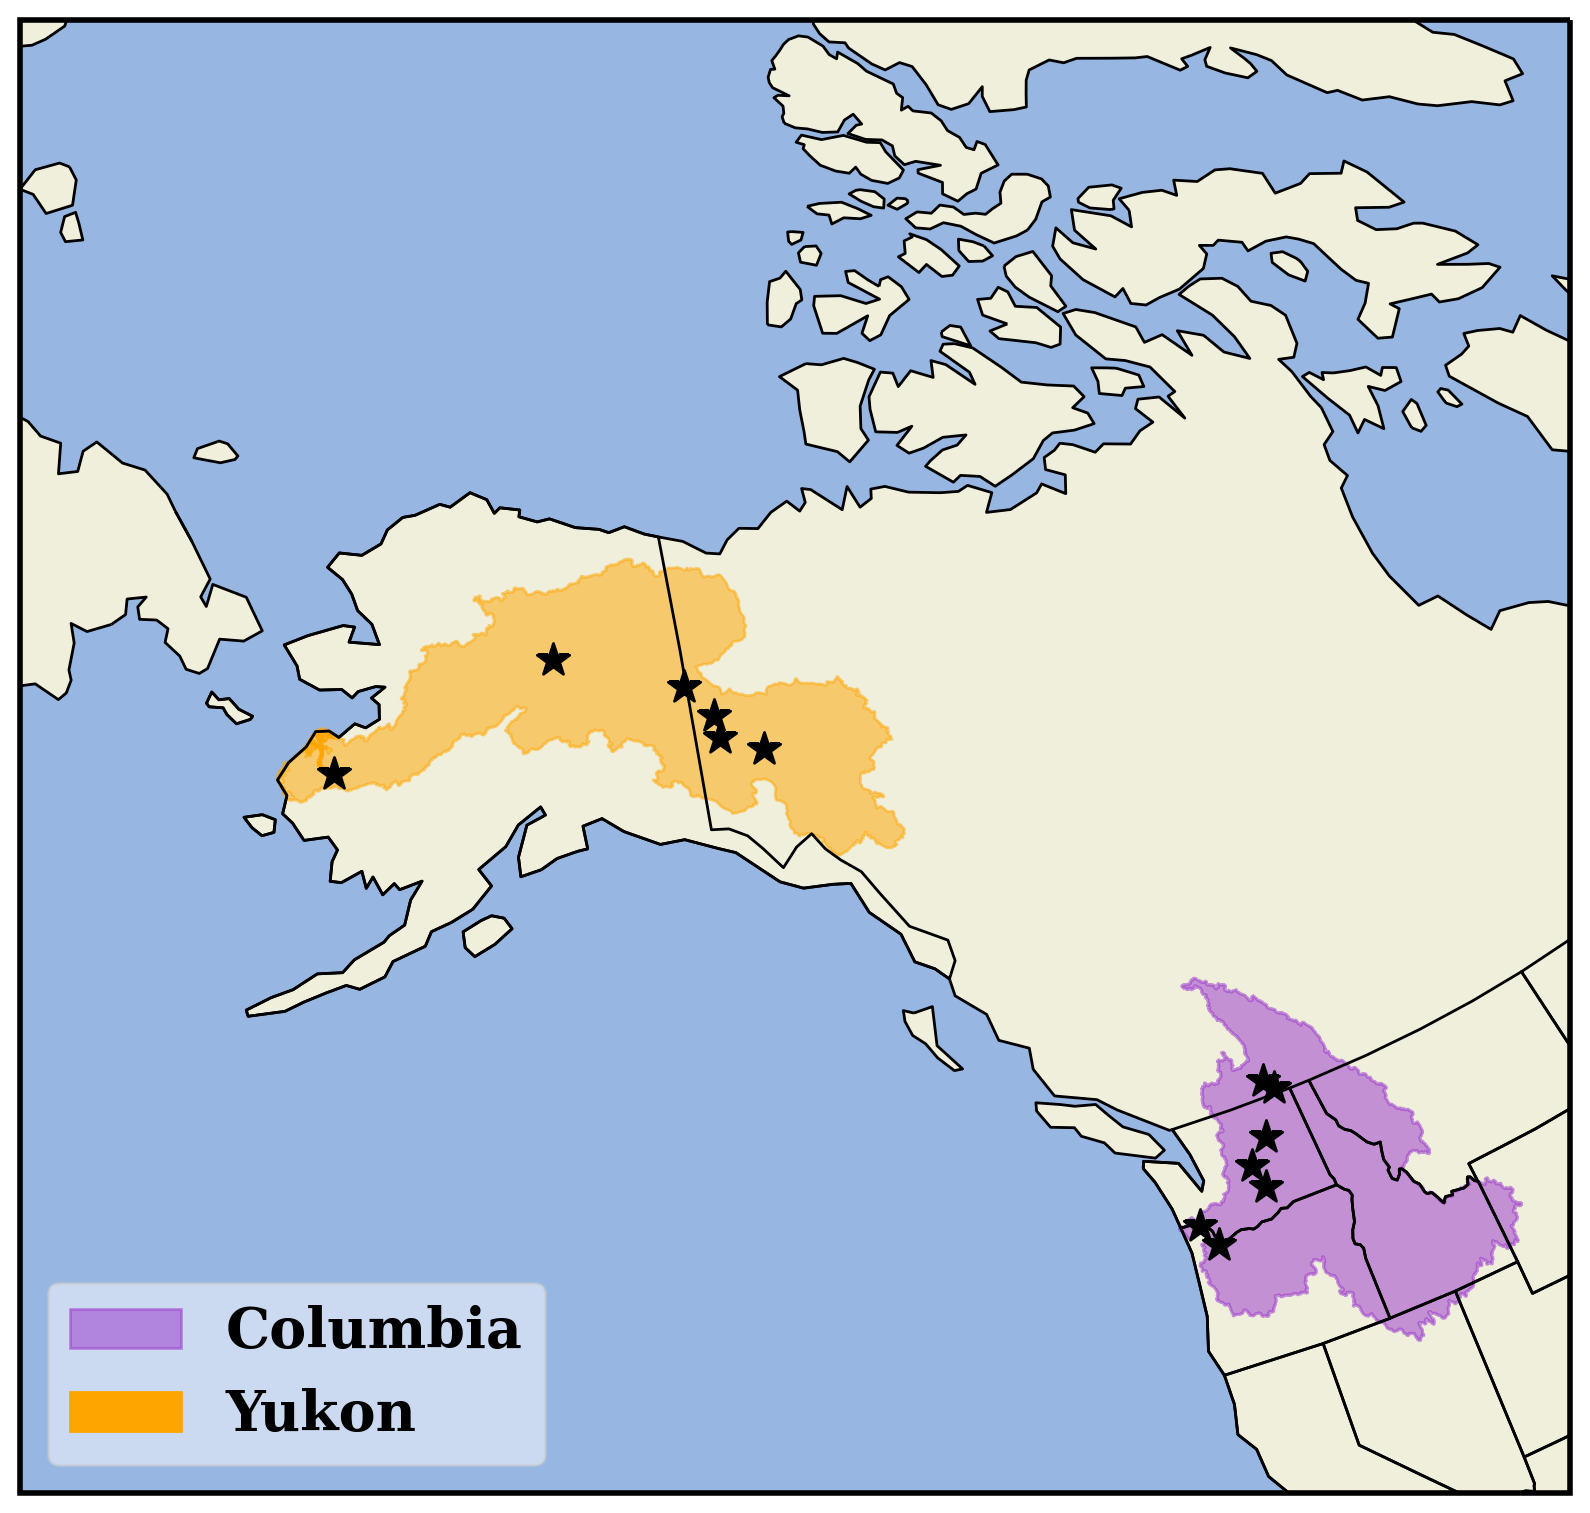
\includegraphics[width=1.0\linewidth]{m3/ims/fig3_1.png}
    \label{fig3_1}
\end{figure}

\begin{figure}[!ht]
	\centering
    \caption{Hydrographs of all gauged streamflow data. Second and fourth plots are zoomed in versions of the same colors in the first and third plots. Both have low discharges whose details are lost amongst the larger portions of the river.}
	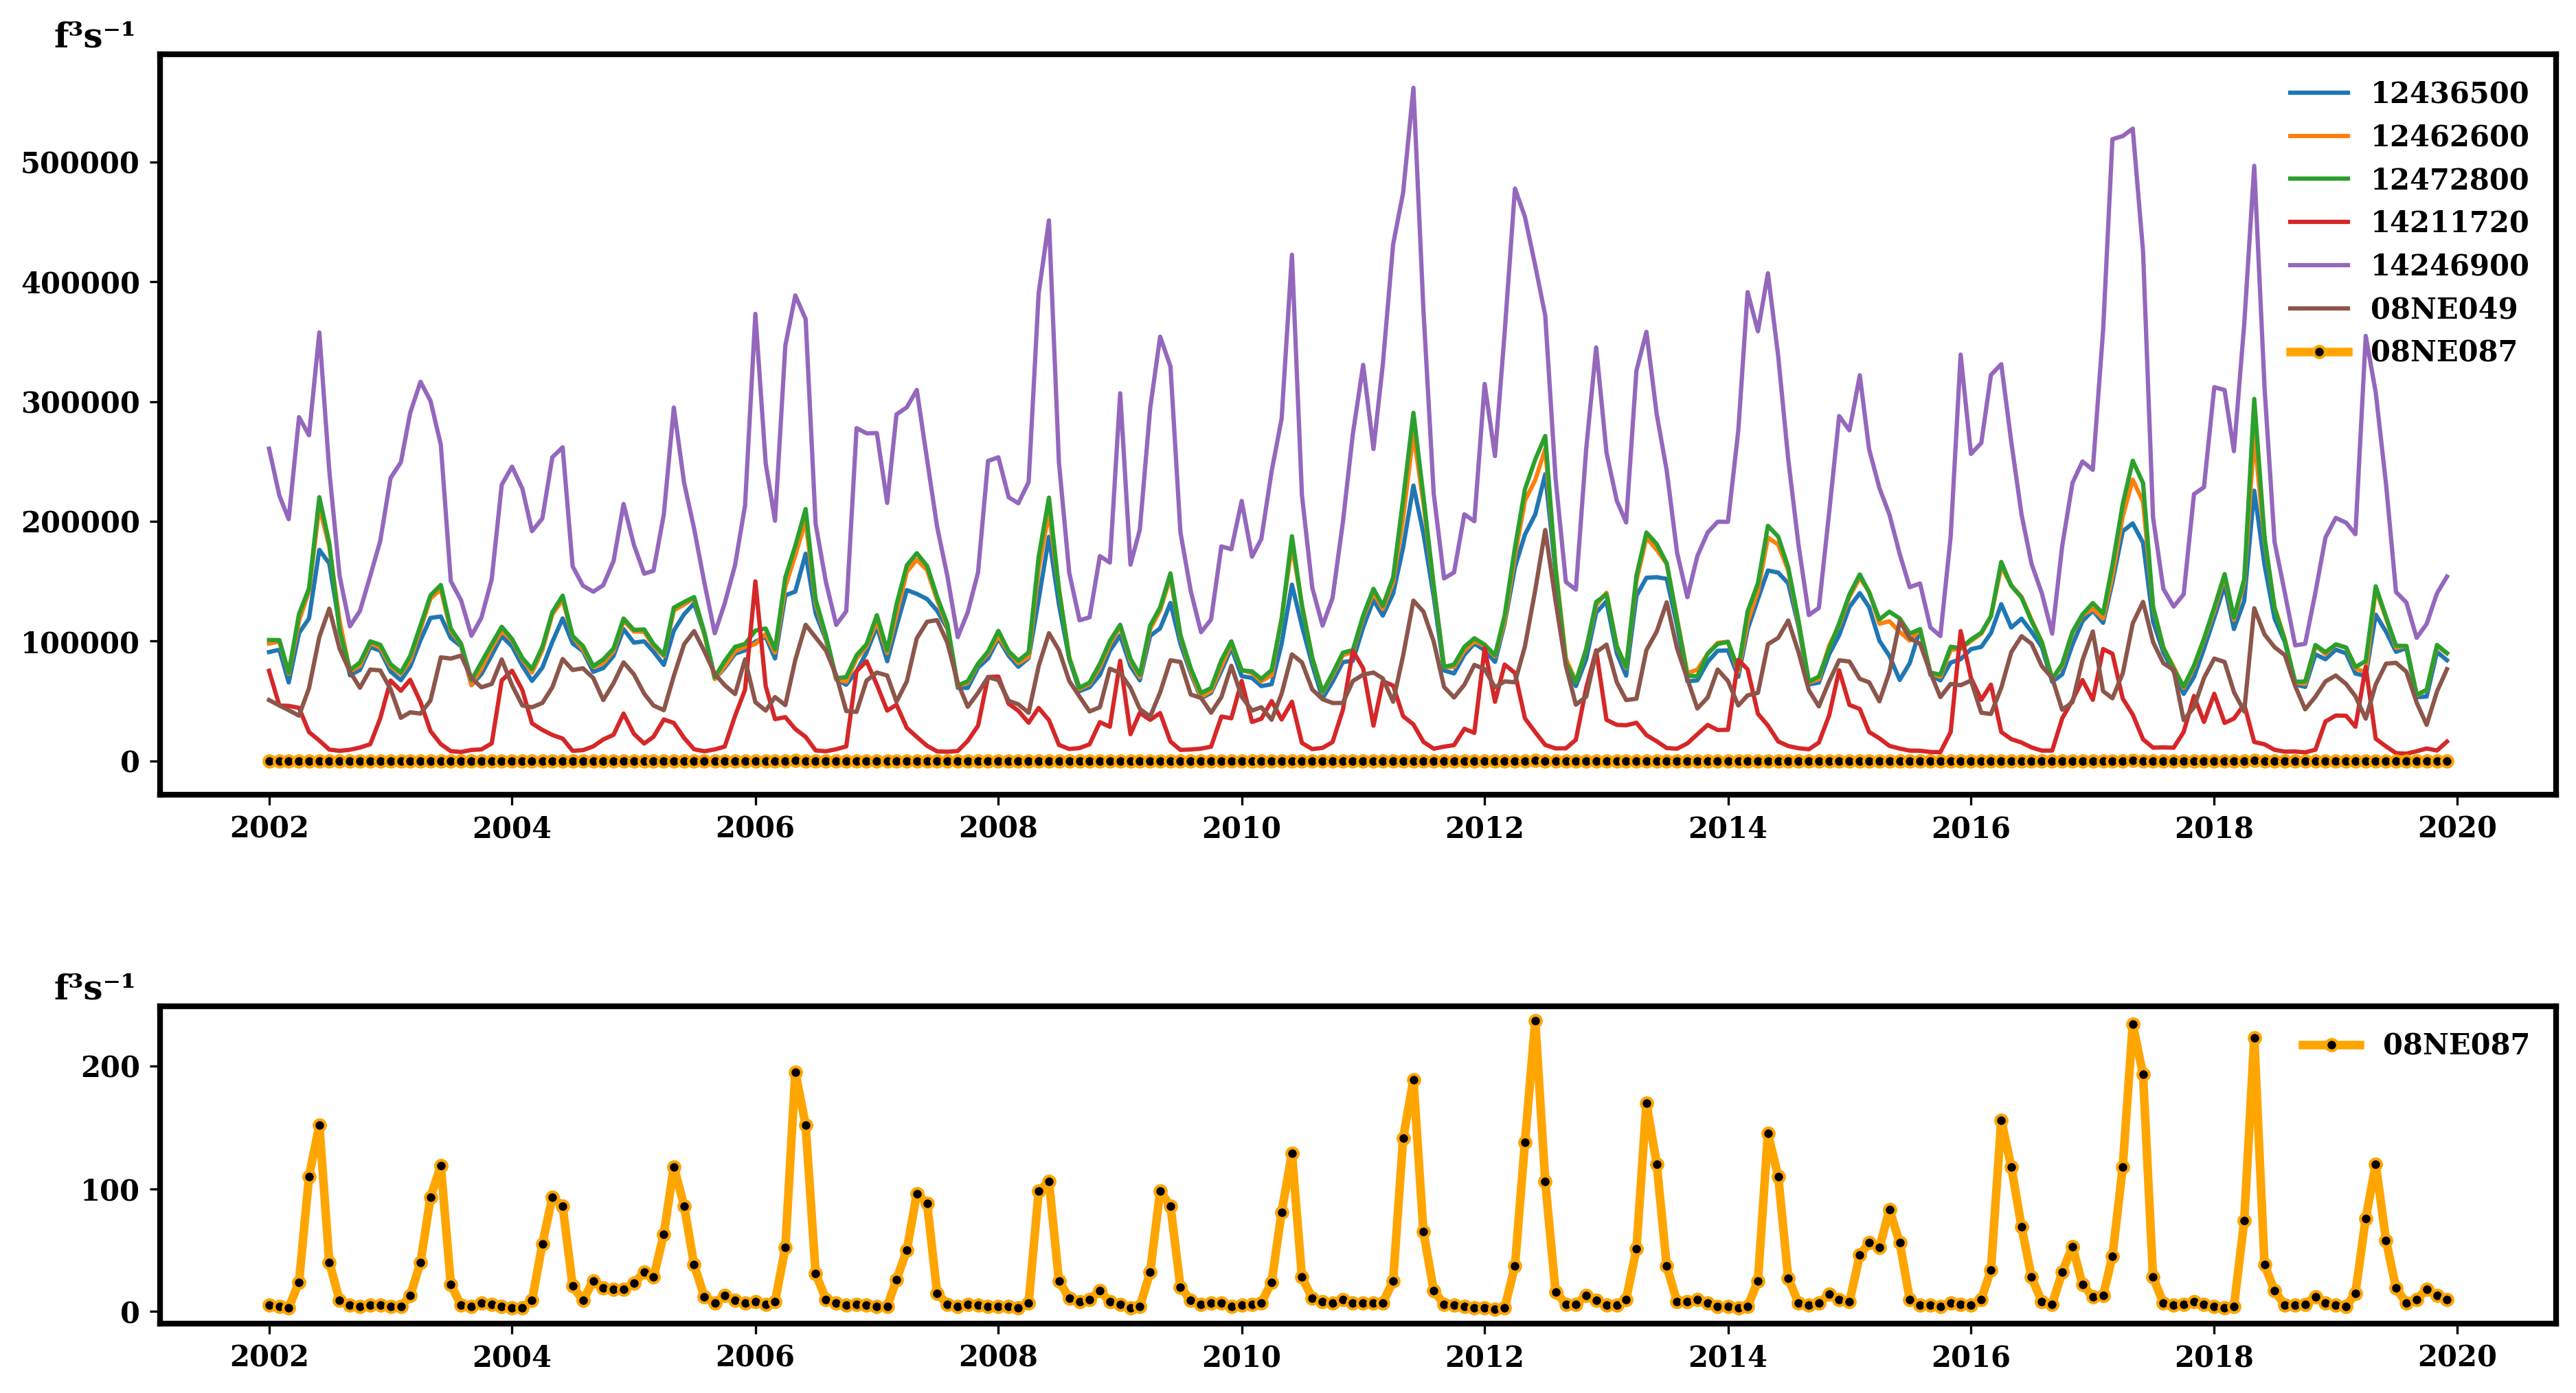
\includegraphics[width=1.0\linewidth]{m3/ims/fig3_2a.png}
    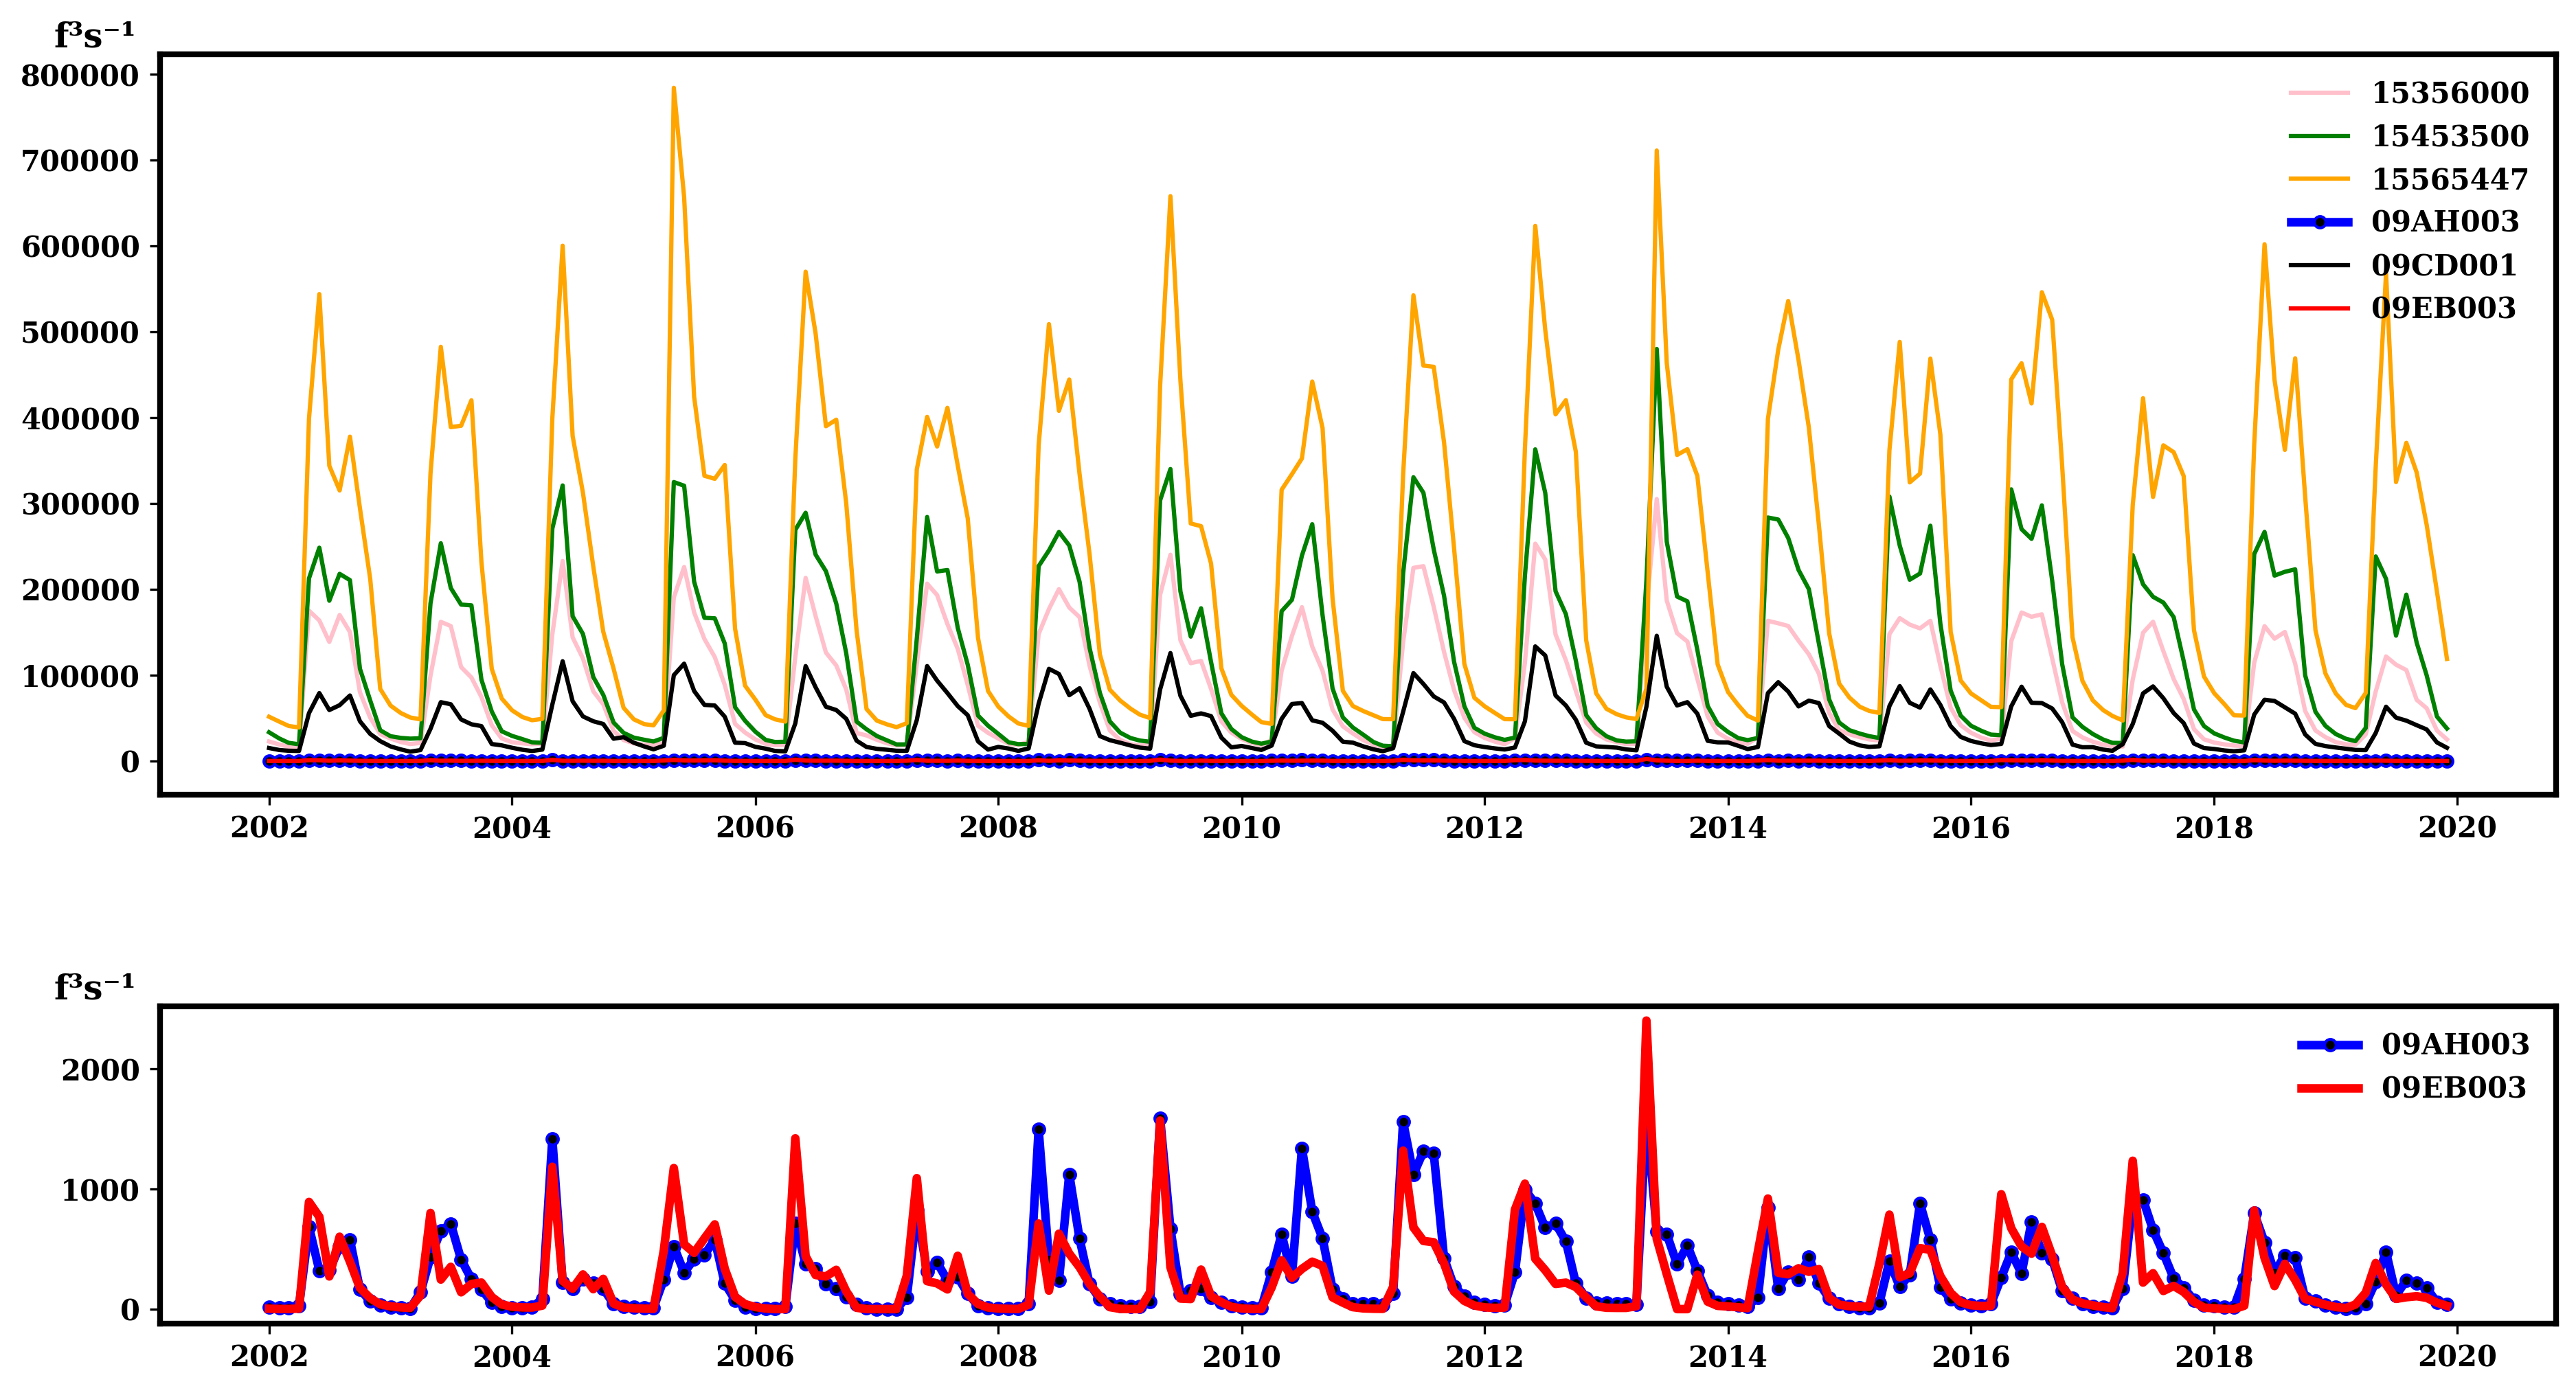
\includegraphics[width=1.0\linewidth]{m3/ims/fig3_2b.png}
    
	\label{fig3_2}
\end{figure}

\begin{figure}[!ht]
	\centering
    \caption{Sample observation of surface flow (Qs), subsurface or groundwater flow (Qsb), Qs + Qsb, flows merged with SST but represented with a single colormap, and flows merged with SST represented with two colormaps highlighting each physical parameter’s unique dynamic range.}
	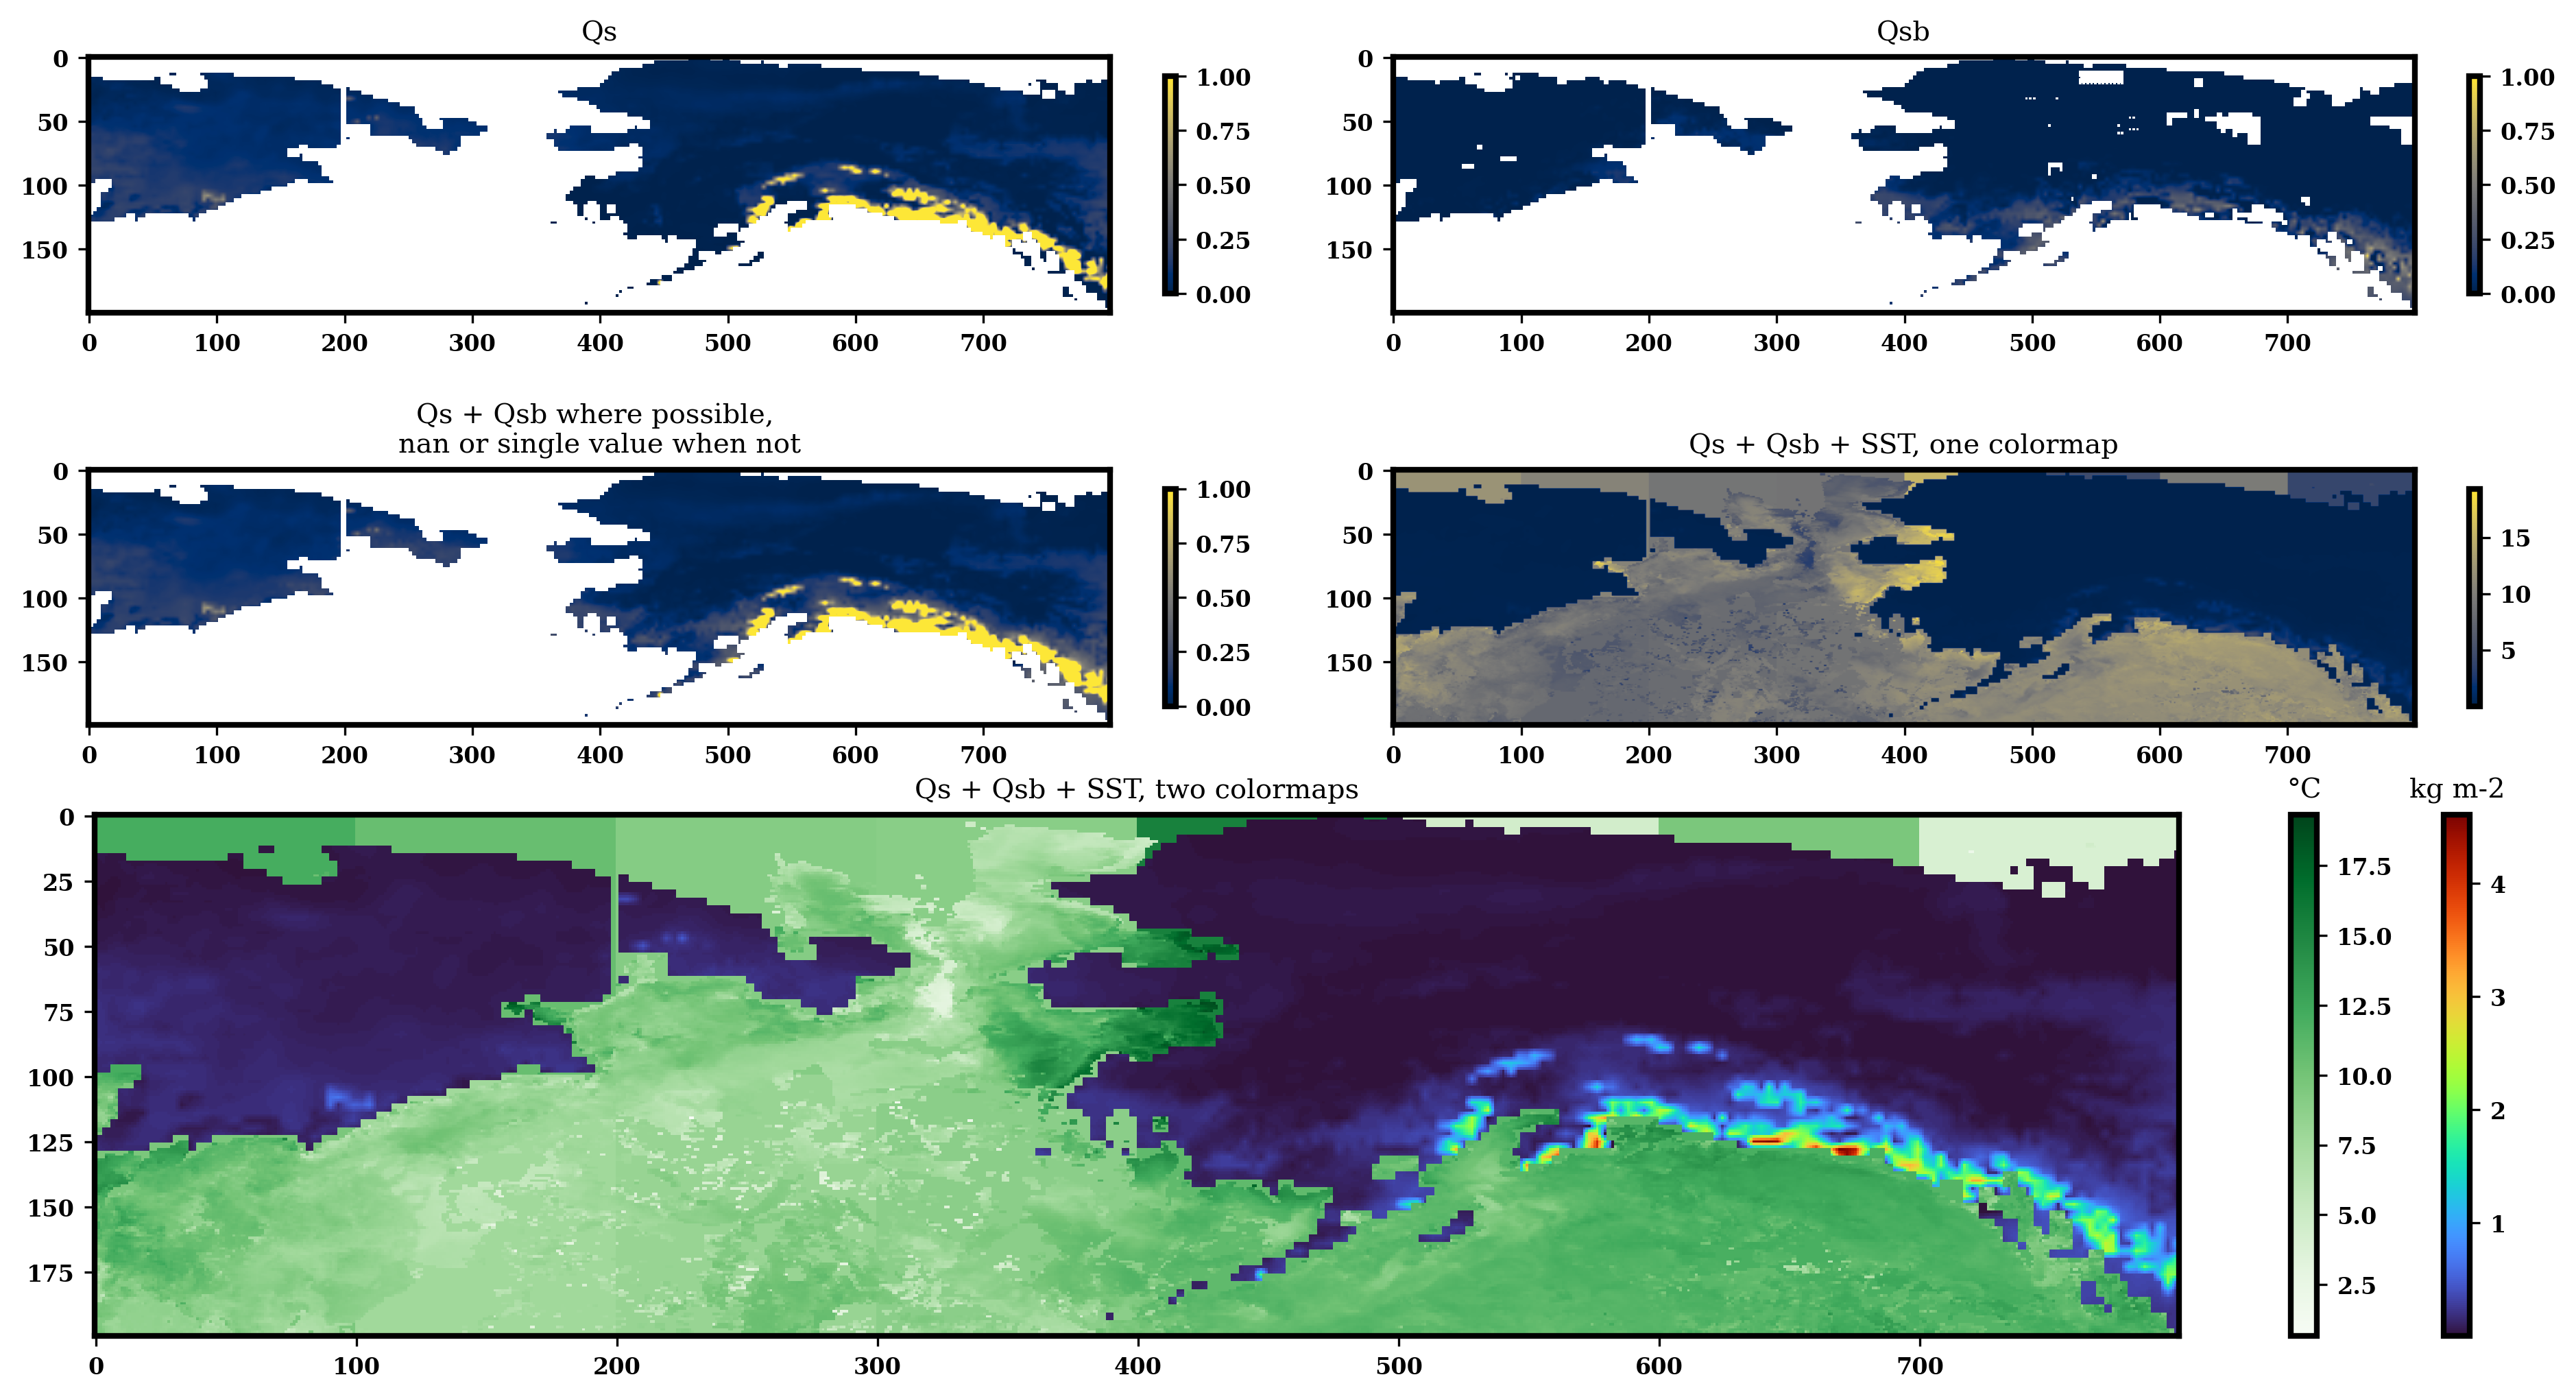
\includegraphics[width=1.0\linewidth]{m3/ims/fig3_3.png}
	\label{fig3_3}
\end{figure}

\begin{figure}[!ht]
	\centering
    \caption{Histograms of model predictability across all experiments delineated by whether SST is included as part of the input or not.}
	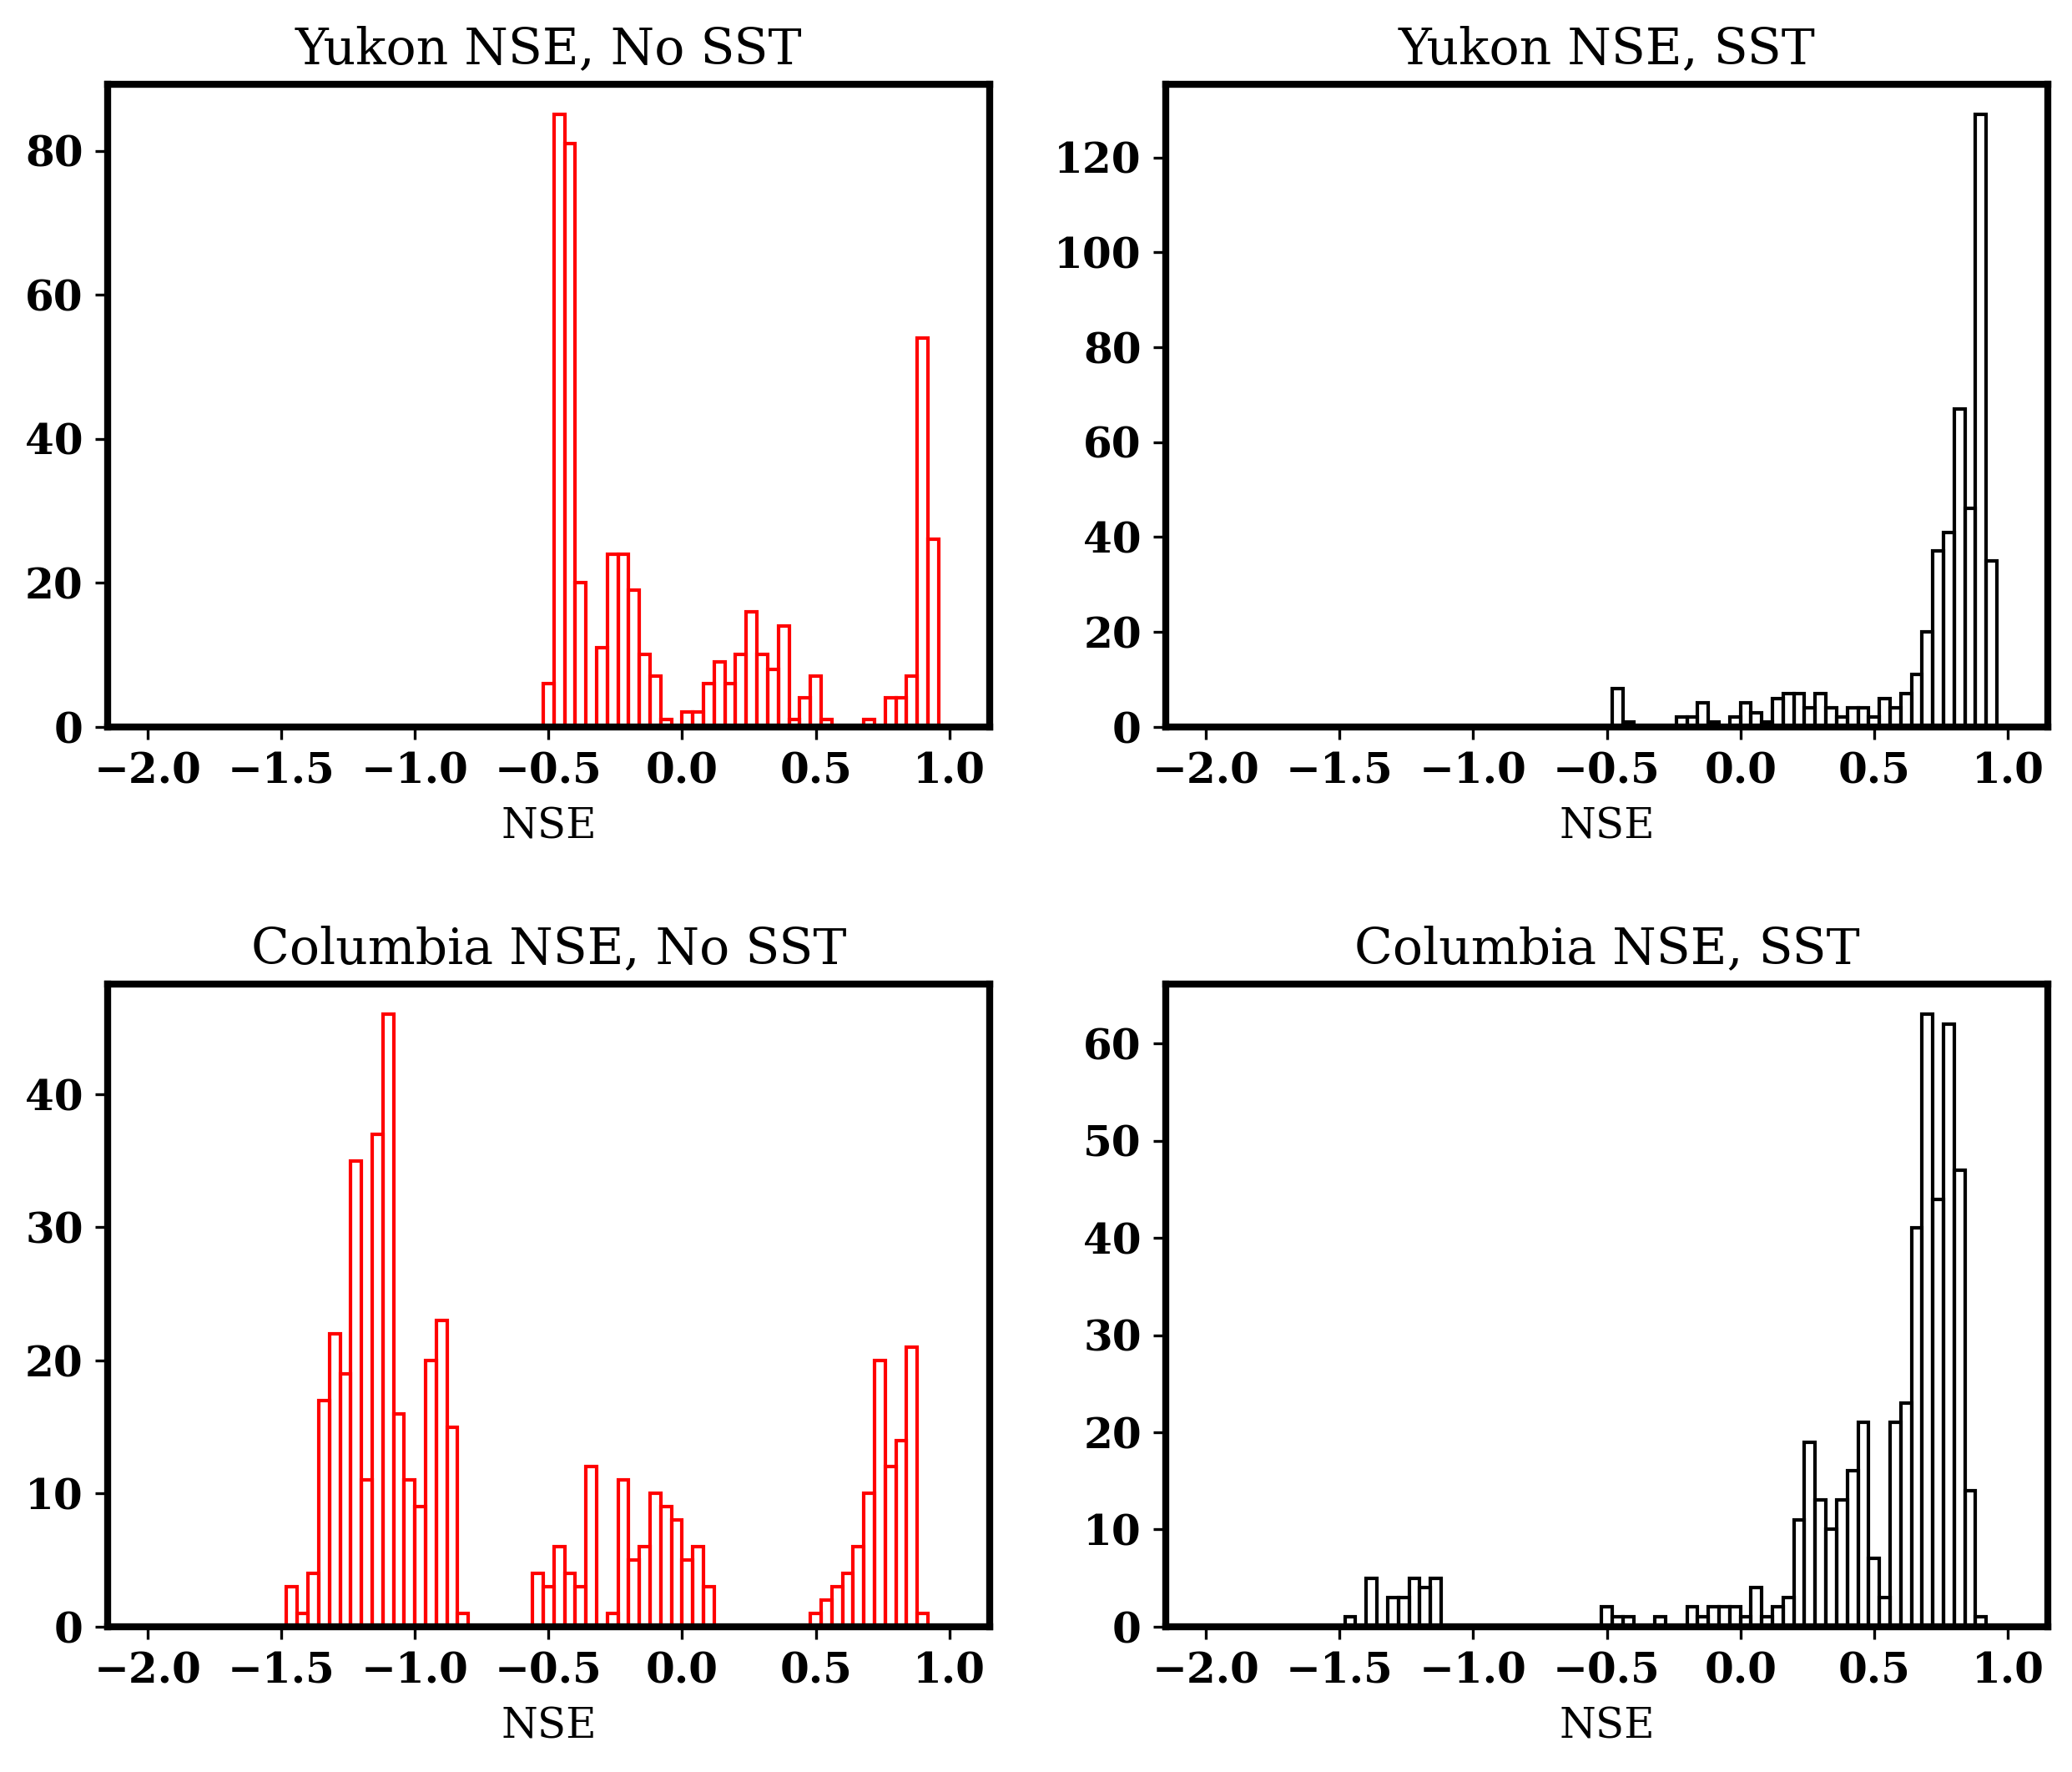
\includegraphics[width=1.0\linewidth]{m3/ims/fig3_4.png}
 	\label{fig3_4}
\end{figure}

\begin{figure}[!ht]
	\centering
    \caption{Histograms of test results for Columbia experiments deconstructed by neural network architecture at the time of training.}
	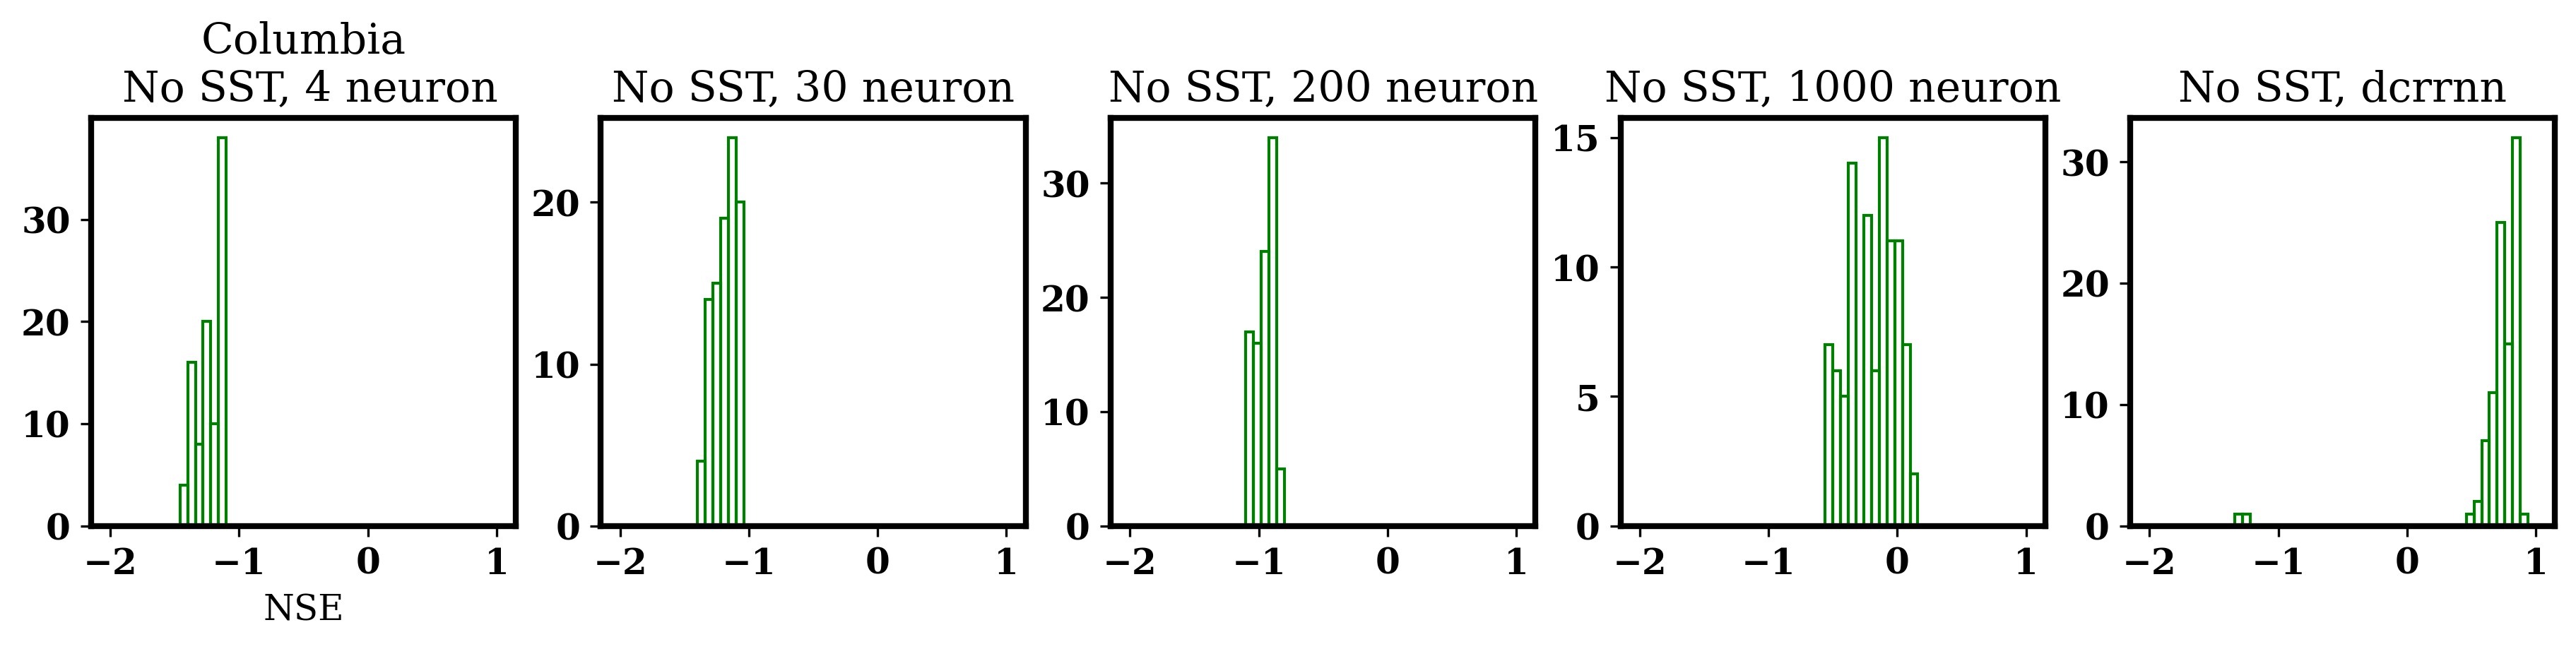
\includegraphics[width=1.0\linewidth]{m3/ims/fig3_5a.png}
    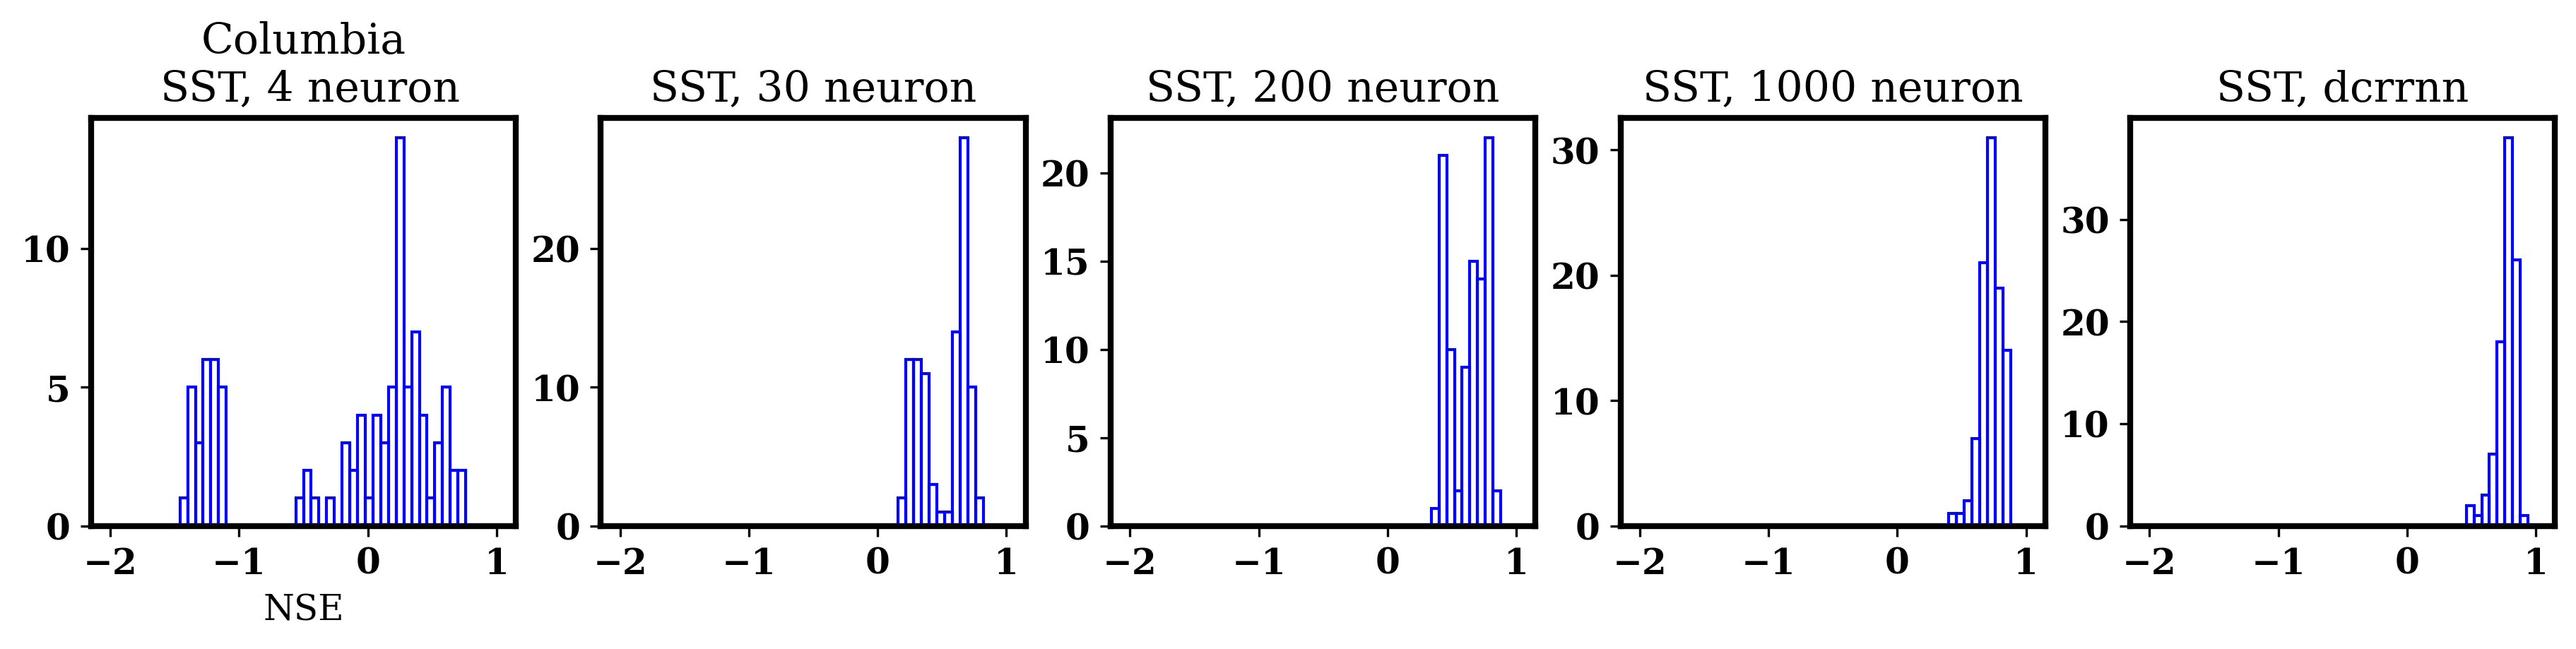
\includegraphics[width=1.0\linewidth]{m3/ims/fig3_5b.png}
    \label{fig3_5}
\end{figure}

\begin{figure}[!ht]
	\centering
    \caption{Histograms of test results for Yukon experiments deconstructed by neural network architecture at the time of training.}
	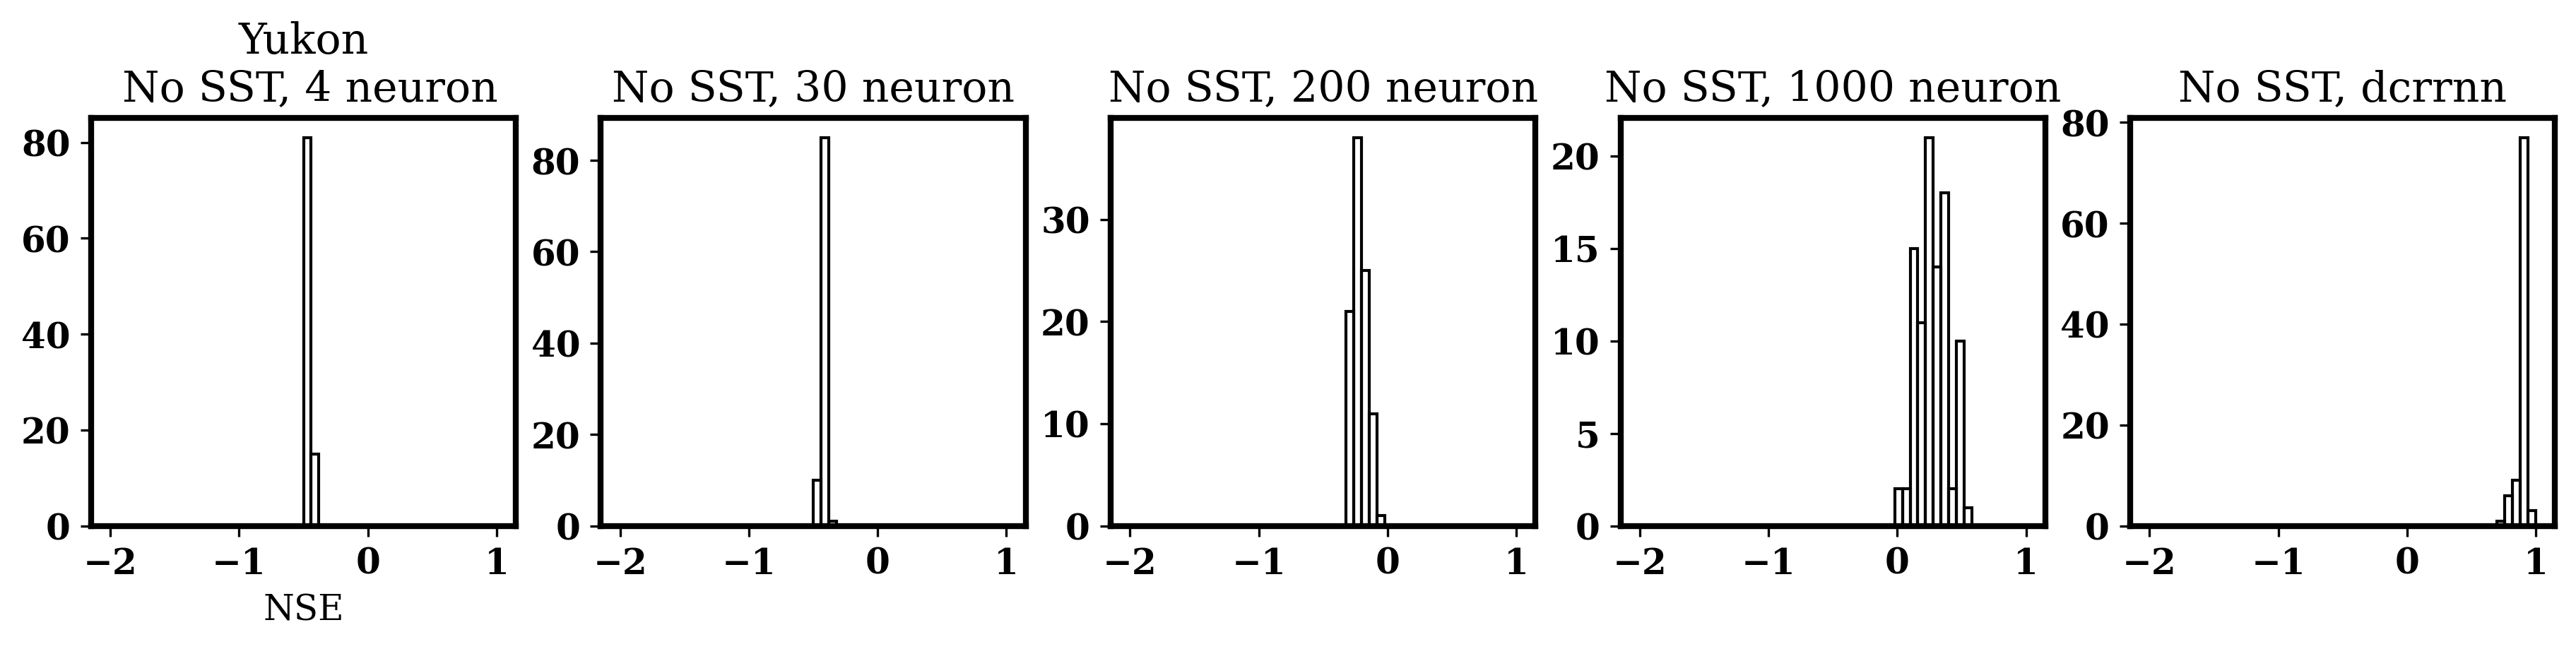
\includegraphics[width=1.0\linewidth]{m3/ims/fig3_6a.png}
    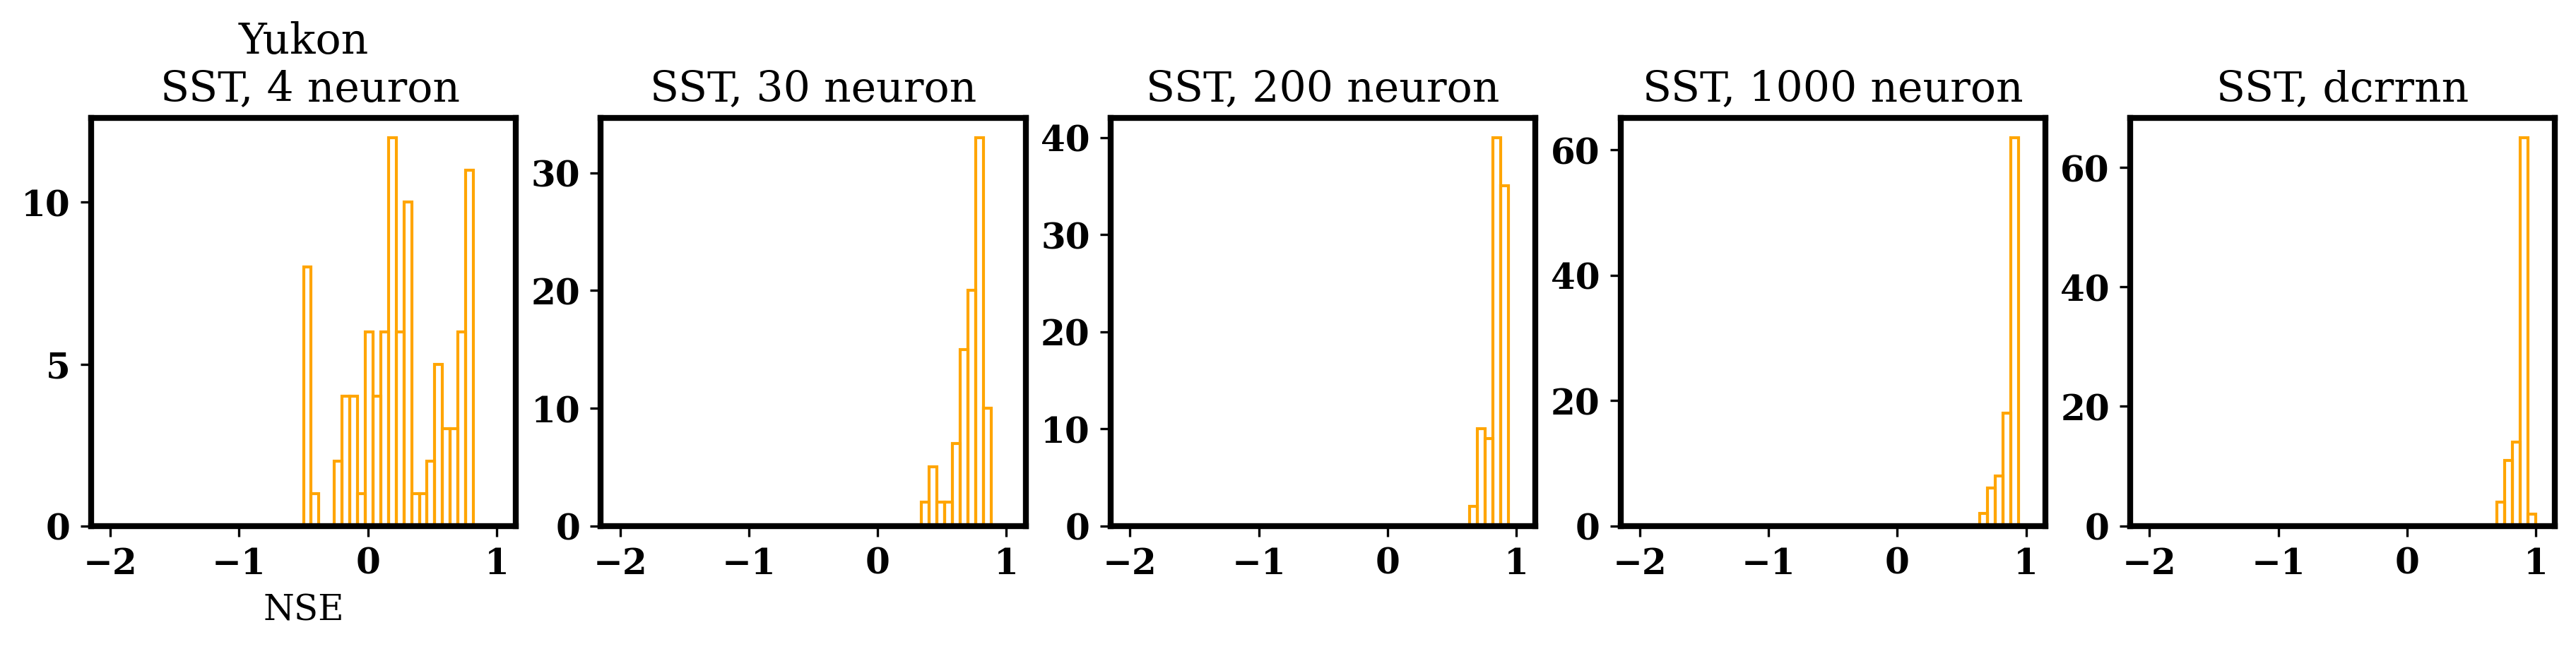
\includegraphics[width=1.0\linewidth]{m3/ims/fig3_6b.png}
    \label{fig3_6}
\end{figure}

\begin{figure}[!ht]
	\centering
    \caption{Columbia \& Yukon experiments using dcrrnn and the 1,000 neuron single hidden layer neural networks, disaggregated by lag.}
	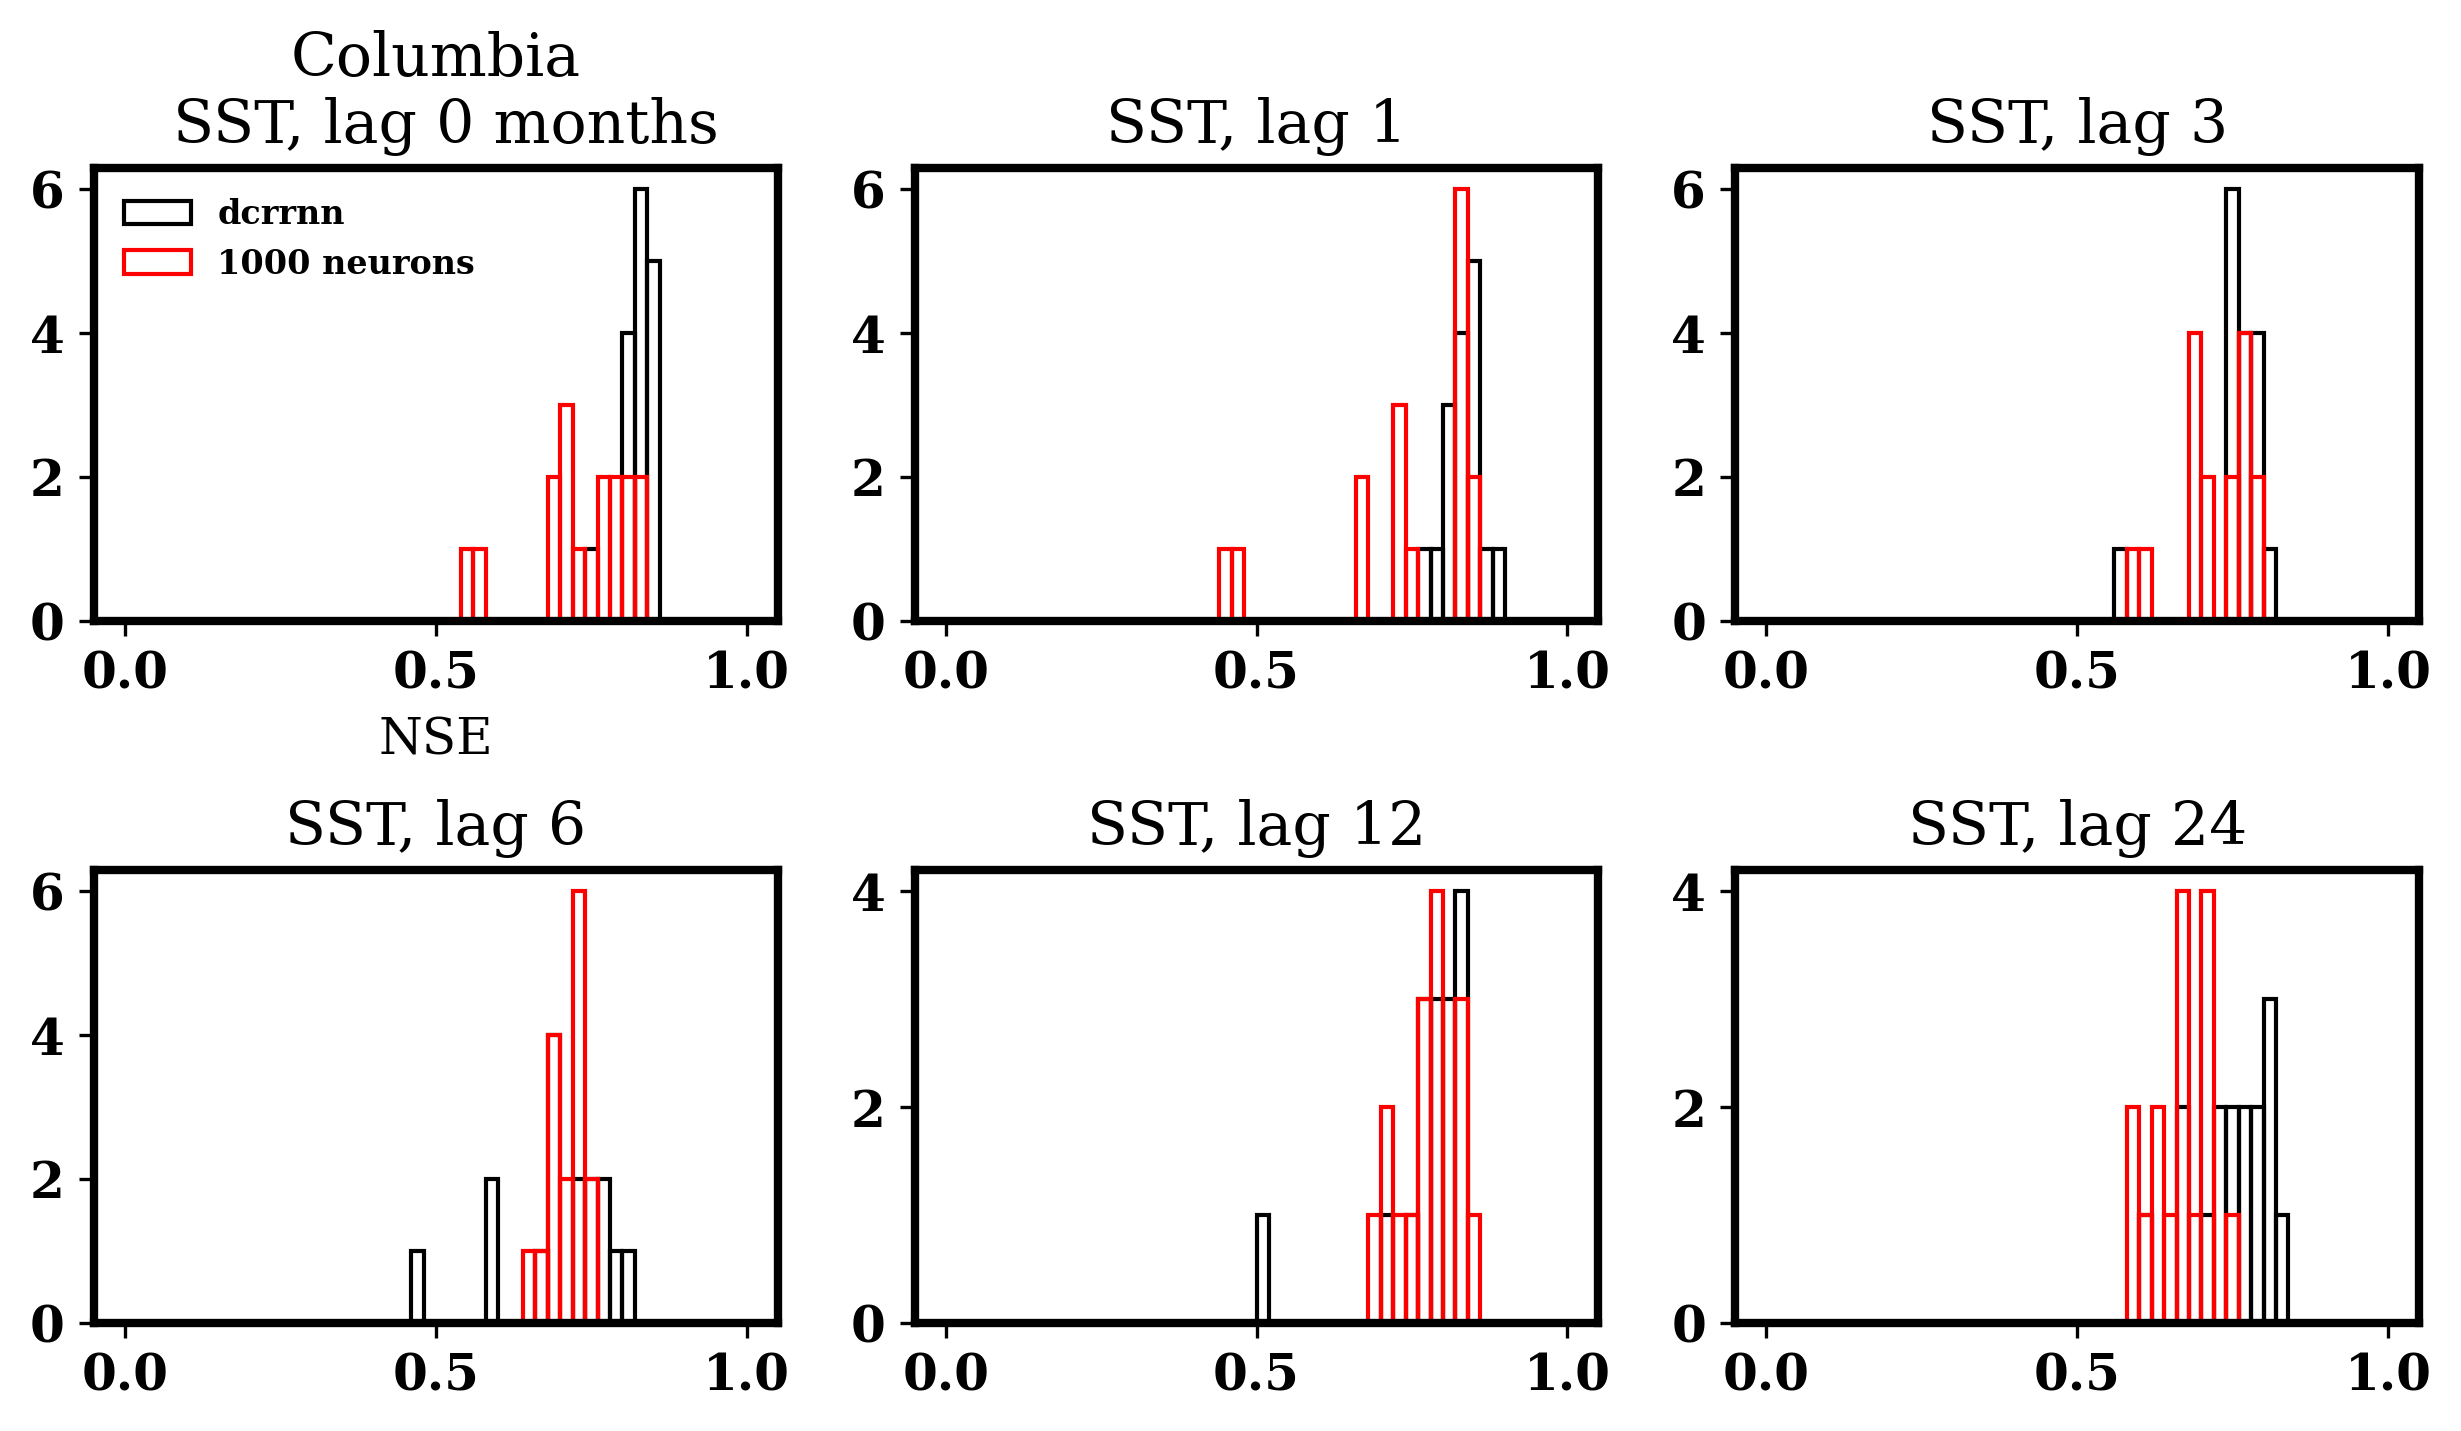
\includegraphics[width=1.0\linewidth]{m3/ims/fig3_7a.png}
    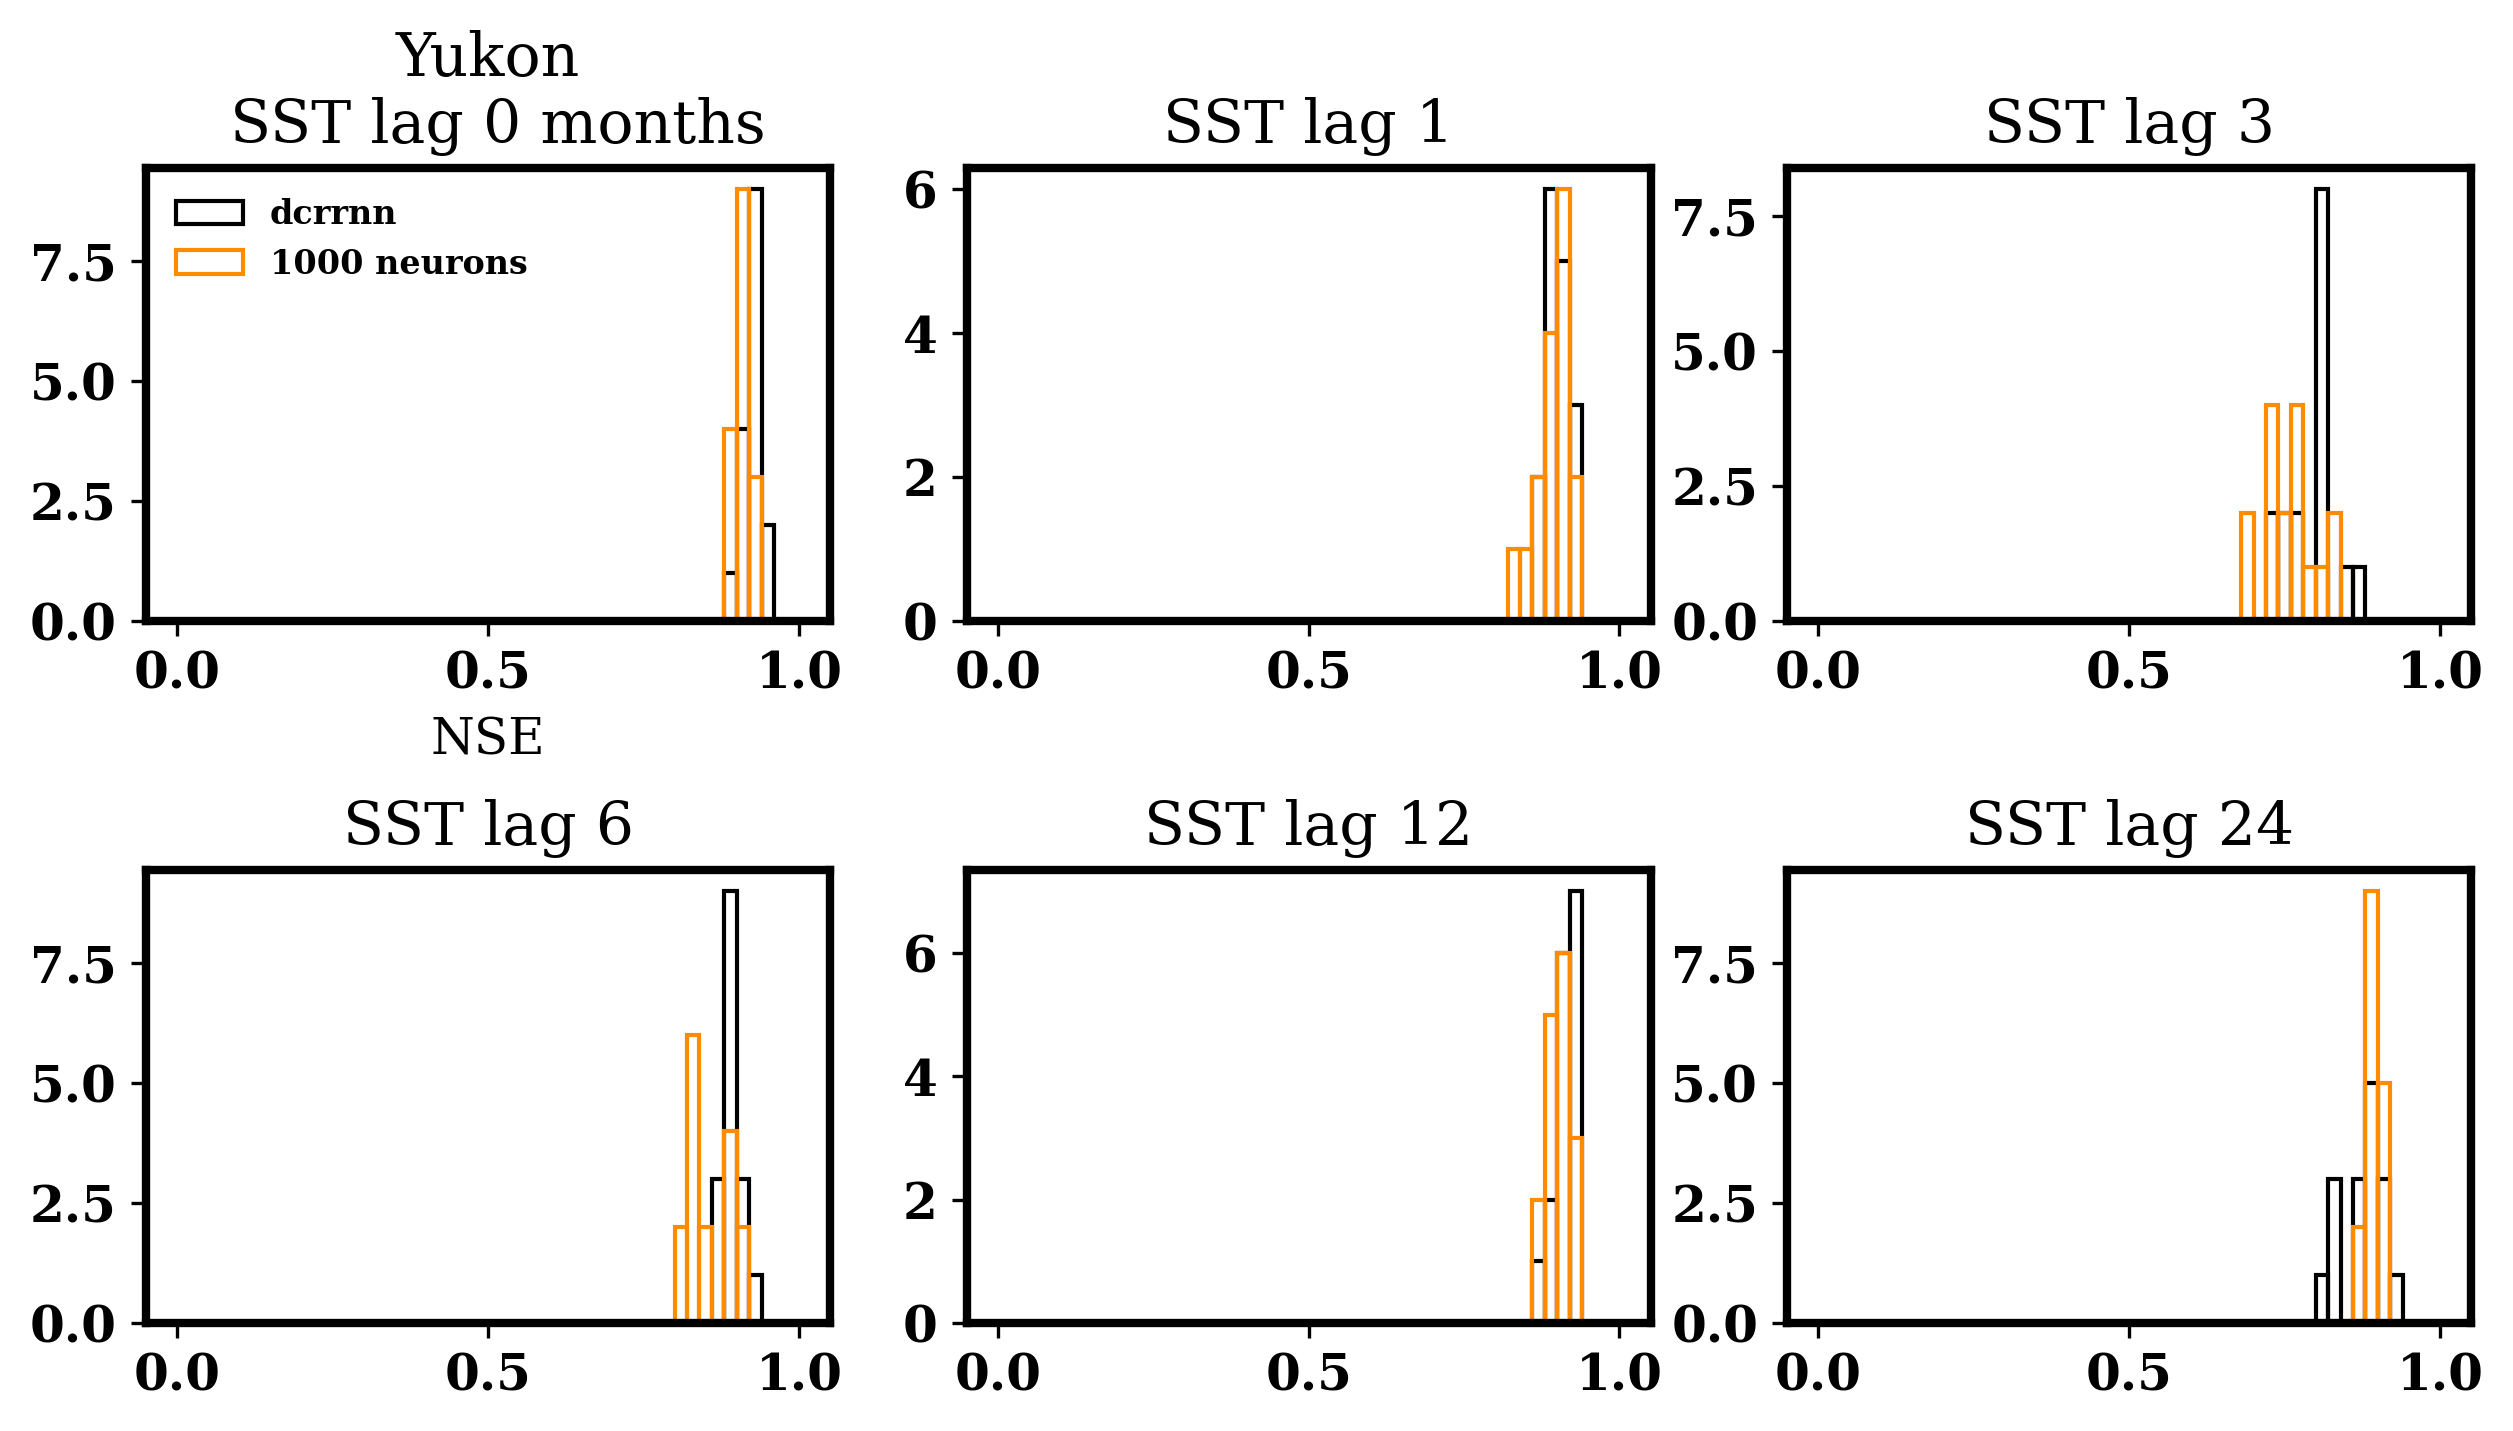
\includegraphics[width=1.0\linewidth]{m3/ims/fig3_7b.png}
    \label{fig3_7}
\end{figure}

\begin{figure}[!ht]
	\centering
    \caption{Columbia \& Yukon experiments using dcrrnn and the 1,000 neuron single hidden layer neural networks, disaggregated by z-scored vs. non-z-scored.}
	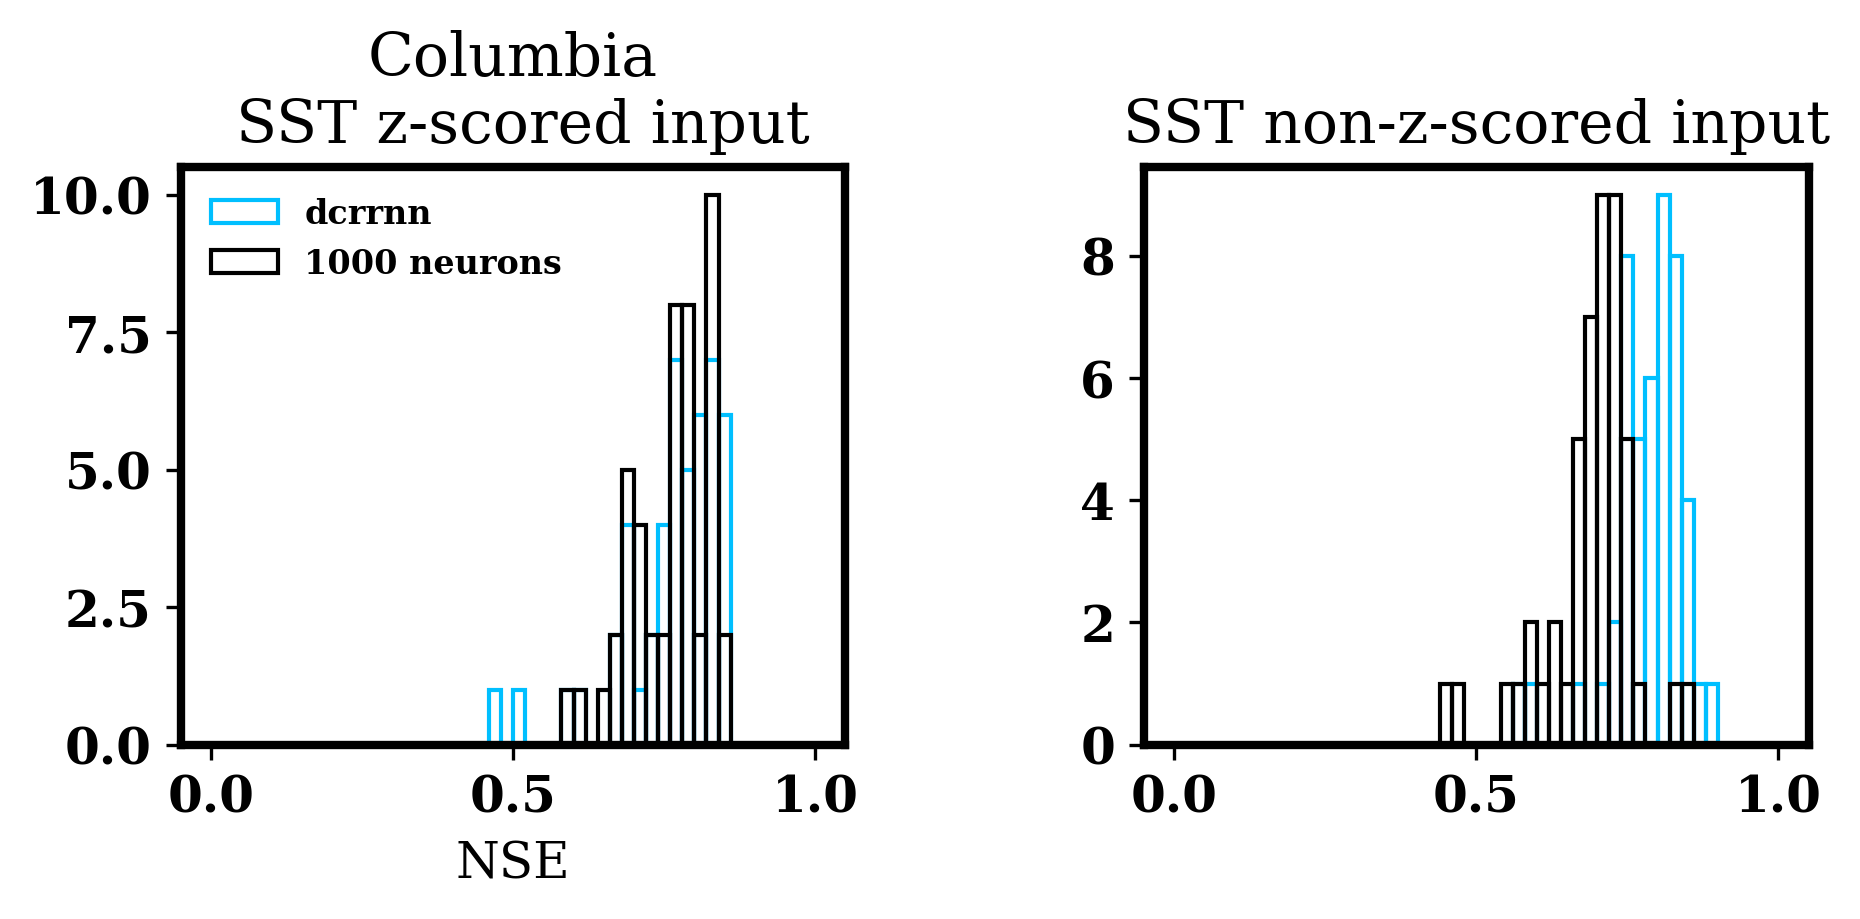
\includegraphics[width=1.0\linewidth]{m3/ims/fig3_8a.png}
    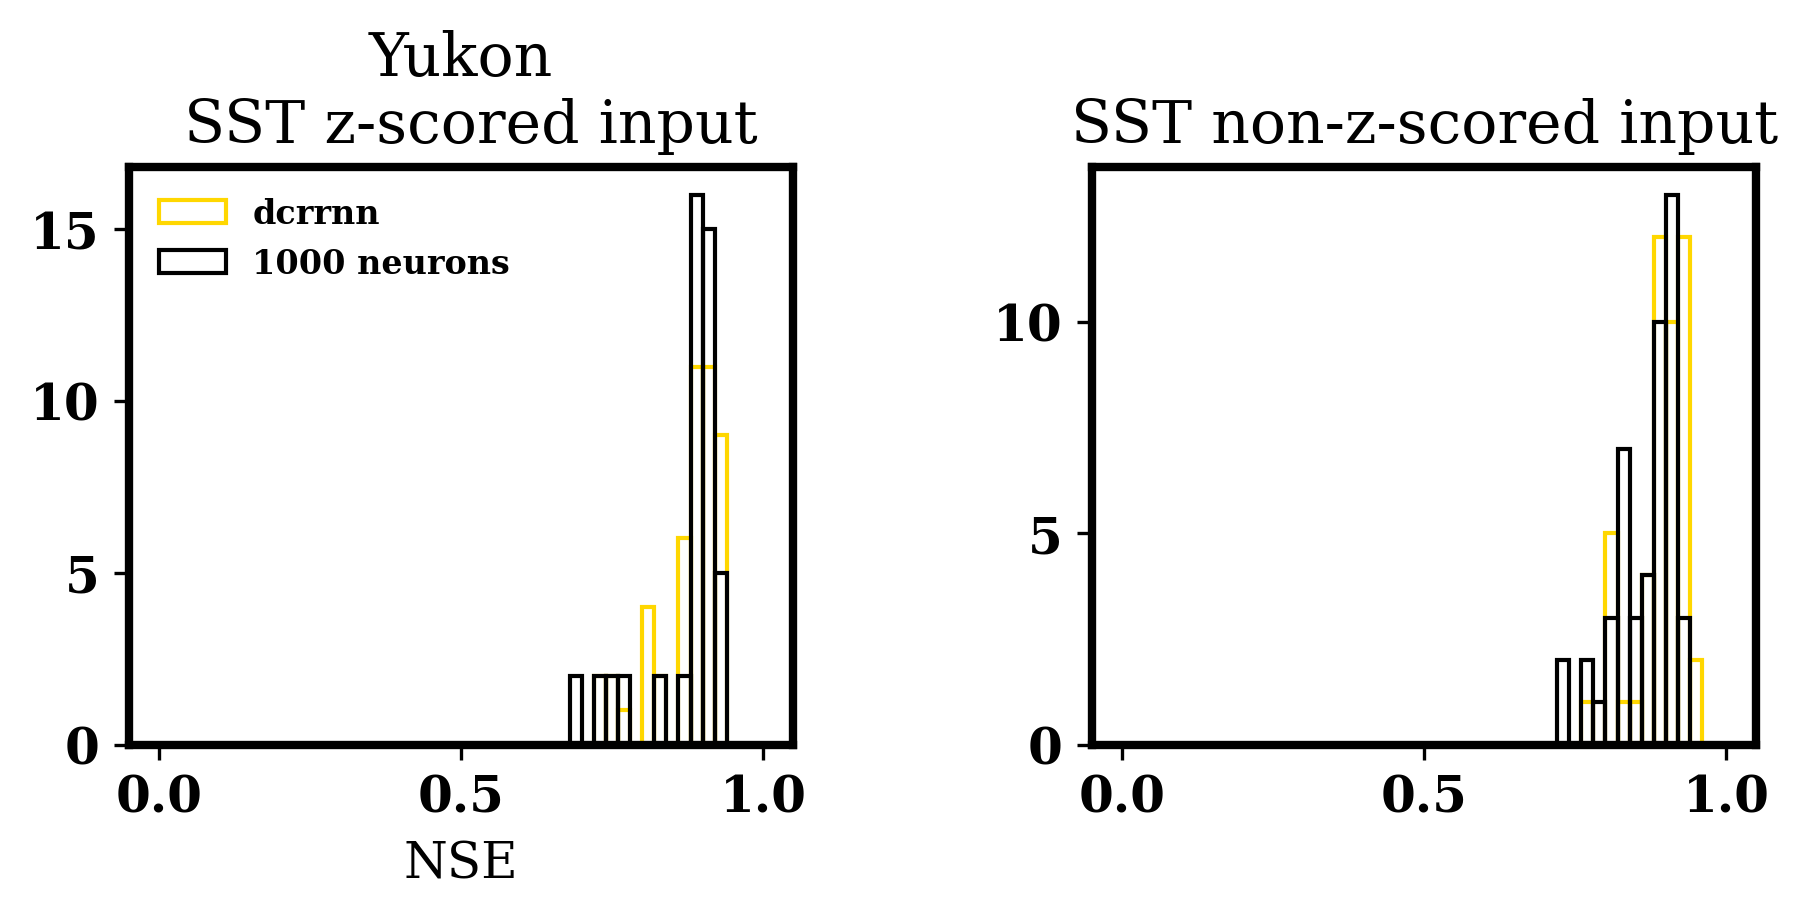
\includegraphics[width=1.0\linewidth]{m3/ims/fig3_8b.png}
    \label{fig3_8}
\end{figure}

\begin{figure}[!ht]
	\centering
    \caption{National Drought Mitigation Center Weekly Output, March 2, 2023, Drought Monitor Output.}
	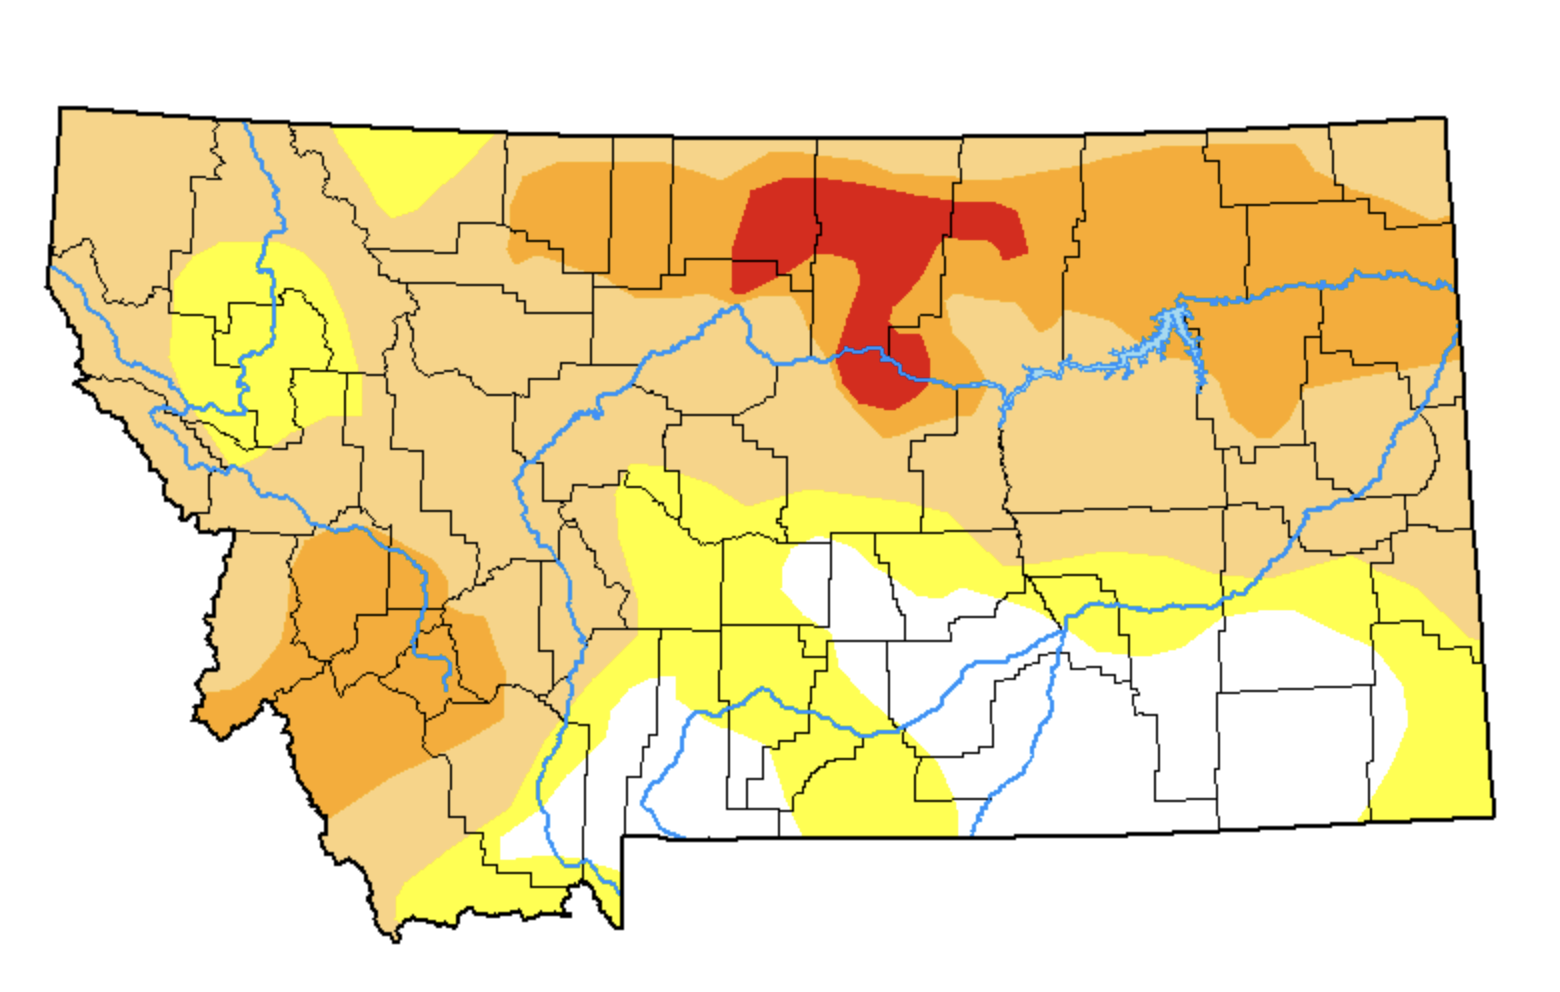
\includegraphics[width=1.0\linewidth]{m3/ims/fig3_9.png}

    \label{fig3_9}
\end{figure}

